%%
%% In the style of a technical report, in 12pt and one sided.
%% Start chapters on right hand side pages only.
%%
\documentclass[12pt]{report}    
%%\documentclass[12pt,twoside,openright]{report} %% Use this for twosided.

%%
%% Load packages.
%%
\usepackage[phd]{otagothesis}     %% Use Otago page layout

\usepackage[longnamesfirst,round]{natbib} %% Use Natural Sciences bibliography

%%\usepackage{times}              %% Times PostScript font. Don't use
				  %% if thesis contains lots of math.

\usepackage{graphicx}             %% jpg, gif, tiff, and pdf graphics
\usepackage{moreverb}             %% Verbatim Code Listings
\usepackage{amssymb}
\usepackage{amsmath}
\usepackage{amsthm}
\usepackage{stmaryrd}
\usepackage{algorithm}
\usepackage[noend]{algpseudocode}

\theoremstyle{definition}
\newtheorem{definition}{Definition}[section]

%%
%% Set title, author and date.
%%
\title{A Suggested Thesis or Dissertation Layout}
\author{Nathan Rountree}
\date{9 February 1998}

%%
%% The library want to know all sorts of personal stuff!
%% Can be left out if you don't use the \frontstuff command
%%
\fullname{Nathan Rountree}
\department{Department of Computer Science}
\dob{1 January 1900} %% date-of-birth
\address{111 North Road, Dunedin, NZ}

%%
%% Uncomment to just print up a few chapters.
%%
%%\includeonly{literature,conclusion}

%%
%% Go!
%%
\begin{document}

%%
%% Put in titlepage and contents, etc...
%%
%\frontstuff

%%
%% Set to one-and-a-half line-spacing
%%
\linespread{1.3} \normalsize

%%
%% Include each chapter as a separate file.
%% These lines assume there are files called intro.tex, literature.tex etc.
%%

%\chapter{Outline}
\label{outline}

\citet{campbell16}

MAKING SOME CHANGES TO TEST GIT WORKFLOW

The focus of the thesis is on the use of information and probability theory measures to track the pose, shape, and appearance of non-rigid articulated objects with multiple independently moving cameras. We demonstrate a hierarchical framework that uses the same independence measure, the HSIC, to estimate first the shape and appearance, then the pose, then the activity of the dominant actor. At each level different features are employed, however the same kernel function and the same Hilbert-Schmidt norm are used to estimate the independence. 

The most elementary level involves a single static camera tracking a single moving non-articulated, rigid object. This requires only that the appearance and the shape be tracked (from here the term appearance will refer to both the appearance and the shape, which are almost always included together). This example is essentially TLD, which is a very robust and accurate tracker. I have made a contribution to show that my algorithm is an extension to TLD in this case. My tracker models a target as a collection of points. Each point is naturally endowed with x, y coordinates. The features for each point are the intensity at that pixel and the distance to the nearest edge. In each frame we find the set of points that maximises the HSIC with the reference (as well as maximising the self similarity and minimising the similarity with the negative training example).

The next case involves rigid-body articulated objects. I show that an articulated object can be viewed as a collection of points that maintain mesh geodesics at all times. In each frame we obtain the prior locations of all the points using optical flow, then perform local optimisations that solve both stage one, with the added geodesic feature. The run time of the algorithm can be improved by computing only the geodesics between points that lie on joints. Note that enforcing geodesic constraints is analogous to analysis-by-synthesis approaches. I believe that it is more useful to use optical flow to approximate the new location of the points, rather than optimising for the model position. I might need to: optimise the 3D model position that maximises the dependence between the two 

\begin{enumerate}
\item{\textbf{Introduction}}
  \begin{enumerate}
    \item{Mixed reality}
        \item{Pose, shape, appearance}
        \item{Articulated objects}
        \item{Markerless motion capture}
        \item{Appearance modelling}
        \item{Activity recognition}
        \item{Independently moving cameras}
          \end{enumerate}
\item{\textbf{Hilbert Schmidt independence criterion}}
  \begin{enumerate}
    \item{Euclidean spaces}
        \item{Functional analysis}
        \item{Hilbert spaces}
        \item{Reproducing property}
        \item{RKHS}
        \item{Kernels}
          \item{Covariance Measures}
        \item{HSIC measure}
          \end{enumerate}
\item{\textbf{Information theory}}
  \begin{enumerate}
    \item{Entropy / uncertainty}
        \item{Mutual information}
        \item{Pose estimation}
          \end{enumerate}
\item{\textbf{Appearance tracking}}
\item{\textbf{Pose estimation}}
  \begin{enumerate}
    \item{Bottom-up}
        \item{Top-down: Analysis by synthesis}
        \item{Calibration free - motion parameter estimation}
          \end{enumerate}
\item{\textbf{Activity recognition}}
  \begin{enumerate}
    \item{Temporal synchronisation}
      \item{Dynamic time warping}
        \end{enumerate}
\item{\textbf{Activity recognition}}
\end{enumerate}


The focus of this thesis is to examine the use of information and probability theory measures to track the pose, shape, and appearance of non-rigid articulated objects with multiple independently moving cameras. We demonstrate a hierarchical framework that uses the same independence measure, the HSIC, to estimate first the shape and appearance, then the pose, then the activity of the dominant actor. At each level different features are employed, however the same kernel function and the same Hilbert-Schmidt norm are used to estimate the independence. 

The most elementary level involves a single static camera tracking a single moving non-articulated, rigid object. This requires only that the appearance and the shape be tracked (from here the term appearance will refer to both the appearance and the shape, which are almost always included together). This example is essentially TLD, which is a very robust and accurate tracker. I have made a contribution to show that my algorithm is an extension to TLD in this case. My tracker models a target as a collection of points. Each point is naturally endowed with x, y coordinates. The features for each point are the intensity at that pixel and the distance to the nearest edge. In each frame we find the set of points that maximises the HSIC with the reference (as well as maximising the self similarity and minimising the similarity with the negative training example).

The next case involves rigid-body articulated objects. I show that an articulated object can be viewed as a collection of points that maintain mesh geodesics at all times. In each frame we obtain the prior locations of all the points using optical flow, then perform local optimisations that solve both stage one, with the added geodesic feature. The run time of the algorithm can be improved by computing only the geodesics between points that lie on joints. Note that enforcing geodesic constraints is analogous to analysis-by-synthesis approaches. 

It is not yet obvious how to use the model / geodesics / optical flow information. 

1. Specify some initial points in the first frame. (the same as we normally would). In each subsequent frame use a local optimisation with the location given by the optical flow information as a prior. 


I believe that it is more useful to use optical flow to approximate the new location of the points, rather than optimising for the model position. I might need to: optimise the 3D model position that maximises the dependence between the two 

\begin{enumerate}
\item{\textbf{Introduction}}
  \begin{enumerate}
    \item{Mixed reality}
        \item{Pose, shape, appearance}
        \item{Articulated objects}
        \item{Markerless motion capture}
        \item{Appearance modelling}
        \item{Activity recognition}
        \item{Independently moving cameras}
          \end{enumerate}
\item{\textbf{Hilbert Schmidt independence criterion}}
  \begin{enumerate}
    \item{Euclidean spaces}
        \item{Functional analysis}
        \item{Hilbert spaces}
        \item{Reproducing property}
        \item{RKHS}
        \item{Kernels}
          \item{Covariance Measures}
        \item{HSIC measure}
          \end{enumerate}
\item{\textbf{Information theory}}
  \begin{enumerate}
    \item{Entropy / uncertainty}
        \item{Mutual information}
        \item{Pose estimation}
          \end{enumerate}
\item{\textbf{Appearance tracking}}
\item{\textbf{Pose estimation}}
  \begin{enumerate}
    \item{Bottom-up}
        \item{Top-down: Analysis by synthesis}
        \item{Calibration free - motion parameter estimation}
          \end{enumerate}
\item{\textbf{Activity recognition}}
  \begin{enumerate}
    \item{Temporal synchronisation}
      \item{Dynamic time warping}
        \end{enumerate}
\item{\textbf{Activity recognition}}
\end{enumerate}
\chapter{Mathematical Preliminaries}
\label{mathbasics}


The prinicple contribution of this thesis is to demonstate the utility of probability and information theory measures for addressing the correspondence problem in certain computer vision applications. In particular we will examine how the \textit{mutual information} (MI) and the \textit{Hilbert Schmidt independence criterion} (HSIC) can be used to evaluate the relationship between two objects. We begin with an introduction to key concepts in probability theory, then demonstrate how these concepts are central to the development of information theory. We conclude with a discussion of the mutual information. In the following chapter we introduce the reader to Hilbert spaces, then demonstrate how Hilbert spaces relate to earlier concepts in probability and information theory. 

\section{Elements of Probability Theory}

\subsection{Probability spaces}

A probability space is a triple $(\Omega, \mathcal{F}, P)$ where $\Omega$ is a sample, or outcome space, $\mathcal{F}$ is the event space, and $P : \mathcal{F} \rightarrow \mathbb{R}$ is a function that maps events to probabilities. The sample space refers to the set of all outcomes that could occur, while the element $A \in \mathcal{F}$ is a subset of the event space such that $A_i \subseteq \Omega$. The function $P : \mathcal{F} \rightarrow \mathbb{R}$ assigns a value to elements of the event space that describe the likelihood of that event occuring. The probability function must satisfy the following properties (2013grayentropy):

\begin{itemize}
	\item \textit{nonnegative:} 
		\begin{equation}
			P(A) \geq 0, \:\: \forall A \in \mathcal{F};
		\end{equation}
	\item \textit{normalised:} 
		\begin{equation}
			P(\Omega) = 1;
		\end{equation}
	\item \textit{countably additive:} 
		$$\text{If} \: A_i \in \mathcal{F}, i = 1, 2, ... \text{are disjoint, then}$$
		\begin{equation}
			P(\bigcup_{i=1}^{\infty} A_i) = \sum_{i=1}^{\infty}{P(A_i)}.
		\end{equation}
\end{itemize}

The first condition states that probability values must be greater than or equal to zero, while the second and third conditions collectively state that 

In the context of computer vision, for example, the sample space is defined by the application. For a set of images the sample space will change depending on factors such as the width and height of the image, the number of channels used to describe each pixel and the range of values each channel can take. The sample space for the set of 8-bit gray-scale images with a fixed width and height is given by the set of all possible configurations of pixel intensities. 

\subsection{Random variables \& Distributions}

(2013durretprobability)
Given our probability space we define a random variable $\mathcal{X}$ to be a function that maps the sample space to some measure space, often the space of real numbers, i.e. $\mathcal{X}\: : \: \Omega \rightarrow \mathbb{R}$. The random variable $\mathcal{X}$ is then said to induce a distribution on $\mathbb{R}$ by letting the probability that $X = a$ be the measure of the set $\{\omega \in \Omega : \mathcal{X}(\omega) = a\}$, which is denoted by $P(\mathcal{X} = a)$. Intuitively, a random variable is an entity that can take on the value of any element of the sample space with probability given by $P$. Drawing a single sample from a distribution is then akin to selecting a particular value for the random variable, according to the probability space. In this work we will denote by $P(x)$ the probability that $\mathcal{X}$ takes on the particular value $x$, i.e. that $P(\mathcal{X} = x)$. Given two random variables, $\mathcal{X}$, and $\mathcal{Y}$, we can define the joint probability $P(\mathcal{X},\mathcal{Y})$ to be the probability distribution for the set of $N$ ordered pairs $\{(x_i,y_i) : x_i \in \mathcal{X}, y_i \in \mathcal{Y}\}$.

We may choose our random variable to be a gray scale image, for example. In the absence of any domain information it may be the case that every pixel value is equally likely to occur, and therefore we describe our random variable as having a uniform distribution. In contrast, we may assume that our image is drawn from a set of images of the natural world, so that it may contain a plant or an animal. In this case there is some restriction on the particular pixel values that are likely to occur, and we therefore say that our random variable is governed by some unknown probability distribution function that we may wish to know more about. We may be interested in knowing, for instance, whether our image contains a kiwi (reference). In our sample space from which we draw images of the natural world there is a probability function that describes the particular configurations of pixels that give rise to images that appear to be kiwi's. Given an image, we may wish to know whether the distribution that generated the current image is equivalent to the true distribution that generates images of kiwi's. This example is obviously far from trivial, as one cannot simply prescribe a function for describing any and all flightless birds from New Zealand. Describing probability functions and their relationship to each other has been the subject of an extraordinary amount of work. In computer science we typically call this problem pattern recognition, which reflects the fact that our goal is to detect patterns and make inferences on the state of the world. 

\subsection{Moments}

In order to understand probability distribution functions we need a language to describe them. This is achieved by computing the \textit{moments} of the distribution. For a discrete univariate probability density function, with an expected value $\mu_1$, the $n^{th}$ moment of the distribution is given by

\begin{equation}
\mu_n = \sum_{i=1}{(x_i - \mu_1)^{n}P(x_i)}.
\end{equation}

\noindent The expectation value, or first moment, of the distribution is given by

\begin{equation}
\mu_1 = \sum_{i=1}{x_i P(x_i)},
\end{equation}

\noindent which is the sum of the individual elements, weighted by their respective probabilities. For a sample of size $N$ the arithmetic mean is given by 

\begin{equation}
\bar{x} = \frac{1}{N}\sum_{i=1}{x_i}.
\end{equation}

\noindent The second moment of the distribution, is given by

\begin{equation}
\mu_2 = \sum_{i=1}{(x_i - \mu_1)^{2}P(x_i)},
\end{equation}

\noindent which is the expected value of the squared deviation from the mean. For a discrete sample the second moment is defined as the variance and is given by 

\begin{equation}
\sigma = \frac{1}{N-1}\sum_{i=1}{(x_i - \bar{x})}.
\end{equation}

\section{Information Theory}

Since Claude Shannon's seminal 1948 paper "A Mathematical Theory of Communication", the field of information theory has developed rapidly. [Give some examples etc].

%$X = \{x_i\}$ and $Y = \{y_i\}$ from the random variables $\mathcal{X}$ and $\mathcal{Y}$

 Much of the early work concerning information theory was intended to be used to develop methods for telephony, and in particular to understand theoretical limits for which a message could be transmitted across a noisy channel. Shannon sought a function that would describe the uncertainty associated with a particular random variable. Shannon recognised that the \textit{entropy}, previously found in statistical mechanics as Boltmann's entropy equation (reference), was a suitable function for relating the probability distribution of a random variable to its uncertainty (\cite{shannon2001mathematical}). For a sample $X = \{x_i\}$ from a random variable $\mathcal{X}$ with corresponding probability distribution $P = \{p_1, p_2, ...., p_N\}$ the Shannon entropy is 

\begin{equation}
	H(X) = \sum_i^N{p_i \: \text{log} \: (p_i)}.
\end{equation}

\noindent Further, \cite{rrnyi1961measures} demonstrated that the Shannon entropy is the limiting case as $\alpha \rightarrow 1$ in a continuous family of functions that satisfy

\begin{equation}
	H_\alpha(X) = \frac{1}{1 -\alpha} \: \text{log}\:\sum_i^N{{p_i}^\alpha}.
\end{equation}

\noindent The Renyi entropy is defined for $\alpha = 2$ as 

\begin{equation}
	\label {renyientropy}
	H_2(X) = - \text{log} \sum_i^N{{p_i}^2}.
\end{equation}

\noindent The joint entropy of the random variables $X$, and $Y$, is given by

\begin{equation}
	H(X, Y) = \sum_i^N\sum_k^N{p_{i,k} \: \text{log} \: (p_{i,k})},
\end{equation}

\noindent where $p_{i,k} = P(x_i,y_k)$ and $Y = \{y_i\}$ is a sample from the random variable $\mathcal{Y}$. One of the key characteristics of the entropy is that it is minimised for events that are either very likely or very unlikely to occur. As a consequence, the entropy is maximised when we are most uncertain about the outcome of an event. Given a Bernoulli trial (such as flipping a coin) the entropy is maximised when the probability of either outcome is equal, as can be seen in (bernoulli entropy figure). 

%\begin{figure}
%	include '~/Desktop/Thesis/Thesis/figureCode/bernoulliEntropy.png'
%\end{figure}

%Note that when $X$ and $Y$ are independent, then we have that $p_{i,k} = p_ip_k$, i.e. that the joint probability of $x_i$ and $y_k$ is equal to the product of their respective probabilities. This means that at independence $H(i,k) = $ 

One of the principle measures to utilise the entropy is the mutual information (reference (shannon?)), defined by

\begin{equation}
	I(X, Y) = H(X) + H(Y)  - H(X, Y).
\end{equation}

The mutual information is the reduction in uncertainty in $X$, given observations of $Y$ (and vice versa). Notably, the mutual information can be used to characterise the dependency between $X$ and $Y$. We can express the mutual information in terms of probabilities as 


\begin{equation}
	I(X, Y) = \sum_i^N\sum_k^N{p_{i,k} \: \text{log} \: (\frac{p_{i,k}}{p_ip_k})},
\end{equation}

\noindent which is zero if and only if $\mathcal{X}$ and $\mathcal{Y}$ are independent, i.e. if and only if $p_{i,k} = p_i\:p_k$. 

We can see that the mutual information will be greater when the respective entropies are maximised and when the joint entropy is maximised. Consider, for example, the outcome of two Bernoulli trials, such as flipping two coins $\text{T}_1$ and $\text{T}_2$ in succession. In order for the mutual information to be maximised we wish to reduce our uncertainty about the outcome of $\text{T}_2$ after observing $\text{T}_1$ by as much as possible. This occurs when our initial uncertainty, i.e our uncertainty about the outcome of $\text{T}_1$, is maximised and our uncertainty about $\text{T}_2$ given $\text{T}_1$ is minimised. We can see that this occurs, for example, when $P(\text{T}_1 = \textit{heads}) = 0.5$ and $P(\text{T}_1 = \textit{heads}, \text{T}_2 = \textit{heads}) = 1$ (with all other joint probabilities equal to zero).

In order to compute the mutual information we need a mechanism to compute the probabilities $p_i$. It is common to use either histograms or Parzen window techniques to approximate the underlying densities. Given samples $X = \{x_i\}$ and $Y = \{y_i\}$, the histogram is constructed by tallying the frequency of occurance of each particular value. We then compute the entropy as per \ref{renyientropy}.

We compute the Parzen density estimate of the mutual information according to the framework laid out by \cite{wells1996multi}. The Parzen window technique (\cite{duda2012pattern}) aproximates a probability distribution as a superposition of functions centered on each of the elements of a sample. Any differentiable function that integrates to one can be used in Parzen density estimation. In this work, as in \cite{wells1996multi}, we will use the Gaussian function:

\begin{equation}
	G_\psi(x) = \frac{1}{\sqrt[]{2\pi|\psi|}} \text{exp}\left(\frac{1}{2}x^\text{T}\psi^{-1}x\right),
\end{equation}

\noindent where $\psi$ is an empirically chosen covariance matrix. In order to approximate the entropy we create two new samples $A$ and $B$ from $X$, with $N_A, N_B < N$ their respective sizes. The entropy is approximated according to 

\begin{equation}       
	H(X) \approx H^*(X) = \frac{-1}{N_B} \sum_{x_i \in B}{\log \frac{1}{N_A} \sum_{x_j \in A}{G_\psi(x_i - x_j)}},
\end{equation}

whereby an individual probability is approximated according to

\begin{equation}
	p(x) \approx p^*(x) = \frac{1}{N_A} \sum_{x_j \in A}{G_\psi(x - x_j)}.
\end{equation}

In his paper, \cite{shannon2001mathematical} states that "The fundamental problem of communication is that of reproducing at one point either exactly or approximately a message selected at another point".











































%pose estimation
\chapter{Object recognition}
\label{objrecognition}


The problem of object recognition can generally be divided into two categories, that of image classification (does this image contain the object?) and localisation (where in the image is the object?). The latter naturally extends to tracking, which requires that objects be localised over consecutive frames. In all cases we must be given some form of reference to match. In the problem of classification this is often a class label on images containing the subject of interest. The problem is then to learn a function that will respond in a particular manner to previously unseen images containing that object. Image classification has been dealt with extensively and there exist robust algorithms that achieve very low errors on many classic datasets, for example convolutional deep neural networks (examples?). Although there exist many interesting problems in image classification it will remain outside the scope of this thesis. \\

Image localisation extends classification by imposing an additional spatial constraint on the output. Rather than simply labelling the class of the image, we now require that the location of the object within the image be specified. In the simplest case, the target is defined by a (typically rectangular) template, from which we can extract a number of features. Tracking is then defined as the problem of finding, for every pair of frames in the video, the transformation that minimises the disagreement between templates in successive images.  \\

\noindent State of the art trackers tend to adhere to the following paradigm:
  
\begin{enumerate}
\item{In the first frame, specify the location of the target.}
\item{Given this initial location, train a classifier.}
\item{For each subsequent frame, find the most probable location of the target and update the classifier.}
\end{enumerate}

This approach is beneficial as it removes the need for an extensive library of labelled examples, which is often prohibitive to acquire, and it allows for the classifier to be trained in response to changes in the appearance of the target. One of the most acclaimed tracking algorithms, TLD (tracking-learning-detect), adheres to this online learning paradigm. TLD uses a labelled set of image patches, given by the initial location of the template, from which it trains a classifier. In subsequent frames the output of the tracking process is used to augment the set of labelled examples (both positive and negative) from which the performance of the classifier is improved. Given the initial bounding box location, () sample from the image to generate a number of base classifiers. The input to each classifier is a set of pixels, the locations of which are unique for every base classifier. That is, no two classifiers share any pixel locations in common. This is necessary to ensure the classifiers generate independent predictions. Each of the base classifiers is used to define an ensemble classifier. The ensemble consists of a posterior probability distribution $P_i(y | x)$ with $y \in \{p,n\}$, which defines the probability of observing any base classifier $i$. An observation of a base classifier is found by making comparisons between each of its pixels and concatenating the binary response into a code, $x$. The probability of a base classifier corresponding to a template patch is then defined as $P_i(y|x) = \frac{\#p}{\#p + \#n}$ where $\#p$ and $\#n$ are the number of positive and negative patches respectively that were observed for the given response.\\

For any given bounding box location, TLD then generates a response for each base classifier, which indexes into the ensemble of predictors $P_i(y|x)$. The response to each predictor is summed and the image patch labelled a match if the response is greater than 50\%. For every frame, TLD tests every possible bounding box location across a number of scales and records the response of the ensemble. Every patch that scores above 50\% is recorded as a detected response. The final output patch is the detected response that lies closest to the output of the optical flow algorithm, which estimates the location of the target by finding the median of the motion vectors that originate in the previous bounding box. TLD is a powerful algorithm because it uses the location of the detected response that was accepted as the true location as a further positive example, and uses the detected examples that were not accepted as negative training examples. This means that over time the algorithm learns to discriminate between the true target and patches that lie close to the decision boundary. While TLD demonstrates superior performance on a number of training examples, it is not clear that updating the classifier based on the spatial layout of likely positive and negative examples is correct in principle. In particular, the use of heuristics to determine which samples to use to update the classifier can lead to incorrect patch labelling, which, over time, can cause the classifier to drift. Grabner (2008) address this problem by introducing a prior over likely patch labels, which they use to adapt an online boosting algorithm. Similarly, Saffari (2010) use a combination of multiple views and priors to enforce consistency amongst a set of classifiers. Leistner (2009) focus on developing a robust loss function to improve the classifier learning phase. In contrast, Hare (2011) learn a function that predicts the transformation of the target between frames, rather than training a classifier that will give a binary response on an input patch. Their method, which they term STRUCK, utilises a support vector machine (SVM) to estimate the location of the target in a given frame. They use the output of this estimation process to update the SVM, with additional budgeting constraints to restrict the growth in the number of support vectors. In this manner, STRUCK incorporates the patch labelling decision into the classification and learning process, rather than leaving it as an additional step after classification. 

One of the principle limitations of the methods introduced above is speed. All of these algorithms rely on costly template representations and update strategies. Moreover, the prohibitive speeds affect the number of examples that can be used to update, affecting the overall learning quality. While these trackers can generally be formulated to operate in near real-time, it is possible to achieve significant improvements in speed without major precision sacrifices using \textit{correlation filters}. Correlation filters operate in a similar fashion to the trackers mentioned above, however they make use of the Fast Fourier Transform (FFT, ref) to improve the tracking speed. Given an input image $f$ and a 2D filter $h$, the output of the correlation process is an image $g$. In the ideal case $g$ would be specified by a Gaussian function with a peak at the true target location. The Convolution Theorem states that the correlation can be given by an element-wise multiplication in the Fourier domain (Bolme (2010)). Given the Fourier transforms $\text{F} = \mathcal{F}(f)$ and $\text{H} = \mathcal{F}(h)$ the correlation output is 

\begin{equation}
\text{G} = \text{F} \varodot \text{H}^*
\end{equation}

\noindent where $\varodot$ denotes element-wise multiplication and $^*$ the complex conjugate. The optimal filter given the training examples is 

\begin{equation}
\text{H}^* = \frac{\sum_i \text{G}_i \varodot \text{F}_i^*}{\sum_i \text{F}_i \varodot \text{F}_i^*}
\end{equation}

\noindent where $\text{F}_i$ is a training patch in the Fourier domain and $\text{G}_i$ is the desired response. For a full derivation of this expression please see Bolme (2010). The desired response is taken to be a 2D Gaussian centred on the training patch. The detected response in frame $t$ is used to update the filter, according to

\begin{equation}
\text{H}_t^* = \frac{\text{A}_t}{\text{B}_t}
\end{equation}

\begin{equation}
\text{A}_t = \mu \text{G}_t \varodot \text{F}_t^* + (1 - \mu)\text{A}_{t-1}
\end{equation}

\begin{equation}
\text{B}_t = \mu \text{F}_t \varodot \text{F}_t^* + (1 - \mu)\text{A}_{t-1}
\end{equation}

\noindent where $\mu$ is a learning rate and $\frac{\text{A}_t}{\text{B}_t}$ is an element-wise division. The MOSSE filter demonstrates robust tracking performance on many standard datasets. Notably, Bolme (2010) report a median frame rate of 669 frames per second with a filter of size 64x64 pixels. Correlation filters can be further improved by using complementary cues to develop a robust model of the target. Bertinetto (2015) introduce the STAPLE tracker, which uses two models in parallel to achieve state of the art tracking performance at approximately 90 frames per second. STAPLE outperforms all of the entries in the VOT2014 challenge (Bertinetto 2015) by integrating a colour histogram and a correlation filter with histograms of oriented gradients (HOG) as the features. \\

The principle benefit of correlation filters arises from the fact that they can learn from a large amount of training data while maintaining very high frame rates. In particular, correlation filters are trained on data that can be stored in circulant matrices. A circulant matrix is formed by shifting a data vector by one position and storing the resulting vector as a row in the matrix. Notably, circulant matrices can be diagonalised using Fourier transforms and used to provide a rapid solution in ridge regression. Henriques (2014) introduce a kernelised filter which is obtained as a solution to a ridge regression problem. They demonstrate that under certain conditions the kernel matrix is circulant, and therefore a fast solution can be obtained for large training datasets and non-linear features.  \\

Kernelised circulant correlation filters are fast and can be trained on a large number of training examples. They are limited, however, to tracking objects that undergo minimal changes in pose, for some arbitrary definition of minimal. Tracking performance can be improved by using HOG filters, which are robust to changes in pose, however by definition a square bounding box around an articulated target will naturally include background features. We therefore turn to articulated pose estimation, which takes principles from object recognition and applies them to articulated objects. In particular, we demonstrate how the HSIC can be used to develop an articulated tracker that can learn from very few training examples. Although we have not demonstrated how the results of Henriques (2014) could be applied to our work, we consider hypothetical examples of how this may occur. (is HS-DTW the circulant link?)  


[how does struck perform against TLD? Is it weaker because it's computationally heavy and can't support as many features?]  

[talk about that paper that describes the best trackers].

One of the more subtle benefits of an algorithm such as TLD is that it is invariant to camera motion. This is due to the fact that TLD localises the target relative to the camera reference frame, rather than to a world frame. 










%pose estimation
\chapter{Pose Estimation}
\label{poseEstimation}

In this chapter we discuss our approach to detecting and tracking the pose of an articulated object through a series of images. We begin with a discussion of our approach and demonstrate its performance in a number of different test cases. We conclude with a discussion of prior work in the fields of object recognition, segmentation, and pose estimation. 

\section{Background}

Augmented and virtual reality, which we refer to in this thesis as \textit{mixed reality}, are progressing at a rapid pace. This advancement is due largely to improvements in hardware and in our understanding of the human visual system. Collectively, these advancements mean that mixed reality devices are becoming ergonomic and are capable of delivering content that seamlessly blends with the surrounding world. In particular, this progress means that it is now reasonable to develop mixed reality applications for users interacting in dynamic, unpredictable environments. Consequently, there are two situations for which pose tracking is required. The first is to track the user as she navigates an environment in order to deliver the current pose of the device, necessary for delivering content. The second situation involves tracking both people and objects that occupy the environment surrounding the user. Many mixed reality platform providers (references?) address the first problem (of finding the position of the headset) by tracking the internal dynamics of the headset with embedded inertial sensors. For better performance and for more complex behaviours many providers also require that the user operates within a controlled environment that features a number of cameras around its perimeter. These cameras track the user as they move around the environment, which allows for more interactivity between the user and the application, and improves the positional tracking system within the application, which improves the display performance. In most cases, however, this visual tracking system relies on distinctive visual markers placed on the user. In addition, few systems include capabilities to track external actors. Applications would become far more immersive if mixed reality platforms were capable of tracking arbitrary objects in their environment. 

\subsection{Terminology}

In this thesis we refer to an \textit{actor} as any object, whether it is a person, a car, or a [endemic NZ bird]. We differentiate between the cases where the actor is \textit{rigid} or \textit{non-rigid}, and whether they are \textit{articulated} or not. A human hand, for instance, is a non-rigid articulated object, due to the fact that the fingers can move independently (typically under certain constraints). In contrast, a solid object such as a desk is not articulated (if one ignores any drawers or movable appendages). A human hand is non-rigid because the skin undergoes complex non-linear motions in response to an underlying rigid motion. In this work however we ignore these non-linear effects and treat the hand as a rigid body object. Similarly we treat a walking person as a rigid-body, articulated actor. In the previous chapter we saw that a bounding box could be used to define a template for an actor and to specify its location in the image. This presents a number of difficulties for tracking articulated actors. An articulated actor occupies only a small percentage of the space within a bounding box. By definition, therefore, a filter that tracks an articulated actor will either fail to correctly identify the target, or the classifier will naturally drift as more and more background features are included in the representation. To mitigate these effects we need to use a more natural representation of articulated actors. We therefore use the following definition:

\theoremstyle{definition}
\begin{definition}
\label{articulatedActor}
Given an object represented as a graph over a collection of nodes, the object is rigid and non-articulated if the Euclidean distances between the nodes are fixed. A rigid object is articulated if the Euclidean distances between nodes are free to change, while the Geodesic distances on the mesh remain constant. 
\end{definition}

[actor -> graph -> model]

Actors are represented as a graph $G = (V, E)$. We have that $V = \{v_i\}$ is a set of nodes, $E = \{e_{ij}\}$ is a set of edges and $e_{ij} > 0$ denotes an edge between node $i$ and node $j$. Our graph is weighted, such that that weight on each edge represents the Euclidean distance between it's two nodes, i.e. $e_{ij} = d(i,j)$. The geodesic distances between any two nodes is the sum of the edges that lie on the shortest path between them. Intuitively this works in the same way as a skeleton. At any point in time separate joints that are not connected through a bone may be any aribitrary Euclidean distance from each other. If we were to find the shortest path between the ends of each of our thumbs, however, we would find that the distance we travel along the bones remains constant at any point in time. Given a series of 2D measurements taken from a moving articulated object, Ross (2010) use a probabilistic formulation to reconstruct the most likely graph from the data.

[probably a good place for a diagram]

In order to reduce the complexity of the problem we assume that any actor we wish to track can be specified by a graph $G$ ahead of time. This means that the distances between the edges are fixed, which  This dramatically reduces our search space, as many of the nodes in our graph are now constrained to move in a particular fashion. 

Given a model of the actor, represented as a graph, how do we represent the pose? There are a number of alternative measures for this, such as exponential maps (), quaternions, and Euler angles. We choose instead to use rotation and translation matrices as these are convenient and we are only dealing with small graphs, so we are not operating under memory constraints. 

[Go into more detail about how the model is put together and how the rotation matrices work etc. + homogeneous coordinates.]

We wish to find the current pose of the actor in every frame of the video. We are choosing in this work to rely on top-down approaches, whereby we place a model into the scene and record the degree to which it fits the image. We then adjust the pose of the model in such a way that after a certain number of iterations we can be confident the pose of the model will align with the true underlying actor. 

We begin by specifying the true location of the actor in the first frame, and from this build our initial model of the actor. Evaluating the model at any given pose means sampling, for every point in the model, the image intensity at that pixel, the distance to the nearest edge and the optical flow information at that point. The similarity between any current pose of our model and the set of positive (or negative) examples is given by the Hilbert-Schmidt independence criterion, as outlined in section x. Using the HSIC as a measure of the similarity between two random variables is advantageous as it captures all of the functional dependencies between the two samples. There are of course many other measures we could use for the similarity, such as the normalised cross correlation (NCC) and the mutual information. The NCC is a linear measure, however, and therefore fails to capture non-linear effects such as dynamic changes in lighting. This is significant, as it is not often the case that positive changes in one variable linearly correlate with positive changes in another variable (or negative changes). Changes tend to be subtle and difficult to discern. In theory the mutual information is the most robust measure for capturing and understanding these non-linear dependencies. The mutual information requires, however, that the underlying probability distributions of the sample from the random variable be estimated. This can be both computationally expensive and can lead to errors in the approximation. Notably, to represent a probability distribution with a histogram, we typically need the number of samples to be much greater than both the dimensionality of the features we are sampling and the size of their respective domains. We can refer to this problem as \textit{coverage} (curse of dimensionality?) which refers to the fact that we need enough samples to cover the domain of every dimension, otherwise the probability distribution can be unnecessarily concentrated in certain regions.



[1. curse of dimensionality diagram?]
[2. example of sampling procedure (intensities, edges etc)]
[3. would be good to show example of the energy surface]
[4. do a comparison of different optimisation procedures]


.\\
.\\
.\\
.\\


object recognition chapter\\
what is pose estimation?\\
	- rigid vs non-rigid\\
	- articulations\\


\subsection{Marker-based Tracking}
The most effective mechanism for estimating the pose of an articulated actor is to use fiducial markers. These small markers, placed on specific locations on the body, serve as easy points to track in a multi-camera setup. The points can be easily differentiated from the background and therefore the trajectories of the joints can be reasonably reconstructed given a video. In every frame of the video the positions of the markers can be estimated by applying blob detection to the images from each of the cameras. Smoothness constraints on the motion of the actor allow for correspondences between blobs in consecutive frames to be established, providing the camera frame rate is high enough. The only problems that typically arise in marker based tracking systems are due to occlusions, however this can be easily resolved by increasing the number of cameras available. While marker based tracking systems are fast and reliable, they are often impractical due to the high cost, the need for multiple calibrated cameras, and because they require physical markers be attached to the actor prior to performance capture. Markerless motion capture systems, most of which rely on computer vision principles, are much more extensively studied and allow for a greater range of applications. The principle focus of this thesis is on the use of markerless motion capture systems for pose estimation. 

Why is it that we can't use a bounding box representaion to track articulated objects? Imagine, for instance, that we are using an object localisation framework, such as TLD or STRUCK, and are using only a template of the object learnt in the first frame. Two major problems arise in this paradigm. The first is that our object will naturally occupy only a portion of the bounding box. Tracking a person with their arms outstretched, for instance, requires a bounding box that naturally includes a large background region in the area under the arms. This background region is included as part of the foreground region and therefore affects tracking performance. Such a tracker would almost immediately fail, even if the actor kept her arms in the same relative position throughout the sequence, as the classification process would need to match the initial background (that was included as part of the foreground) with new background regions. We therefore need a tracking framework that allows for regions other than rectangular bounding boxes to be tracked. 


\subsection{Generative Tracking}

The most common framework for pose estimation of articulated objects is known as \textit{generative tracking}, or alternatively as model-based tracking or analysis-by-synthesis (surveys - moeslund, erol, poppe, sigal). Generative tracking attempts to minimise a model-to-image cost function for every frame in the video. The three main components of any generative tracking framework are the choice of model, the cost function, and the optimisation procedure. Popular generative tracking schemes include PoseCut, which jointly segments an image and optimises the pose of the actor in each frame using conditional random fields (). Similarly, (vineet and sheasby) jointly estimate the optimal segmentation, pose and depth of an articulated actor using a conditional random field. Oikonomidis (hand occlusions) demonstrate a generative technique that matches hand poses to edge and colour maps extracted from an image, while simultaneously preventing any two rigid bodies from intersecting. This method therefore solves for the optimal pose in the presence of physical objects that restrict the space of poses of the hand. Elhayek () present an elegant solution for finding the optimal skeletal and camera parameters by introducing a Sum of Gaussians body model (). By jointly solving for both the camera and pose parameters Elhayek are able to track moving targets from multiple moving, and therefore uncalibrated, cameras. This is significant as camera calibration is a costly process that generally restricts multi-camera pose estimation to cases where the relative position between the cameras is fixed, for instance in stereo reconstruction methods. In contrast, methods for monocular target tracking are prevalent, for example Andriluka (monocular2010) which combines a discriminative 2D people detector and a parts based generative tracking framework to track multiple articulated objects with a single camera. Parts based methods are becoming increasingly common as they separate the recognition problem into multiple subcomponents, each of which are theorised to be easier to solve. Kwon (2013), for instance, treat non-rigid objects as a collection of patches. The pose is represented by the topology between patches and an online model is used to learn appearance classifiers for each of the patches over time. Kiefel \& Gehler (2014) use a conditional markov random field to model the local appearance and the spatial configuration of consituent body parts. These studies are an example of bottom-up, or \textit{discriminative} techniques for pose estimation. They are exemplified by a learning stage that constructs a database or model of training examples. 

Pose estimation techniques can be classified as either \textit{generative}, \textit{discriminative}, or a mixture of the two. Discriminative techniques closely resemble object recognition approaches discussed in the previous chapter. They are characterised by an initial training phase, from which a model is learnt that can be used to output likely 3D poses from images. Conversely, generative techniques optimise the pose of a model that best fits an image. Discriminative techniques are therefore sometimes known as \textit{bottom-up} while generative techniques are known as \textit{top-down}. Discriminative techniques are powerful because they can incoporate a great deal of prior knowledge about shape (Agarwal triggs), appearance (Grabner 2006, andrilukar, kiefel gehler) and motion (akhter) of the target. This becomes limiting, however, as offline learning can be costly, it can be difficult to acquire training databases and the algorithm can be prone to overfitting. This is especially problematic for pose estimation frameworks due to the typically high number of degrees of freedom of the actor, for example. Similarly, articulated objects can undergo signifiant appearance changes and often become self-occluded. In contrast, generative techniques require only a simple model of the target and a function that measures the cost of projecting a given pose of the model into the image. Generative techniques can therefore be adapted to a much wider range of problems and have a greater degree of flexibility in dealing with new and previously unseen situations. They obviously suffer, however, from local minima, especially in regions of high clutter, and can be inefficient in monocular camera systems. 


\subsection{Discriminative Tracking}

Perhaps the most representative example of discriminative tracking comes from (2003athitsosestimating), who use a database of synthetic hand images to estimate the 3D pose of a hand in an image. Their database is constructed by generating an extensive range of synthetic hand images, in a number of different poses for each camera viewpoint. Given any input image the distance to the nearest database image is computed from the Chamfer distance between edge maps in the respective images. A similar view based representation was developed by (1998blackeigentracking) who construct a low-dimensional set of basis images by finding the eigenvectors of a matrix constructed from training images. Tracking is then formulated as a least-squares matching problem. Agarwal and Triggs automatically extract shape descriptor vectors from specific pose silhouettes against which they perform regression, using known motion capture joint angles as the desired output. Pose estimation is performed in subsequent frames by passing the sampled shape descriptors through the regression framework to uncover the 3D joint angles. A number of authors have also proposed techniques that estimate temporal trajectories of an actor by matching to known motion databases. In particular, (2015akhter3dpose) develop a prior model of pose dependent joint limits from a motion capture dataset. They then use this prior to help disambiguate between the multiple ambiguous 3D poses that arise from 2D point observations. (2014zhouspatiotemporal) adopt a similar approach, whereby they learn offline a kinematic model from motion capture data which they then fit to sampled trajectories in every frame. (2001rosalesestimating) introduce a technique that allows the 3D pose to be estimated from a number of uncalibrated cameras. They learn a mapping from image features to 2D joint configurations in a number of virtual cameras. The joint 3D structure and camera poses are then estimated from the set of 2D pose hypotheses. They formulate the reconstruction problem as a probabilistic formulation, for which they use expectation maximisation to find a solution.

So far the techniques we have described have largely focussed on a whole-body formulation for tracking. This is suitable in many instances, however tracking performance often suffers when the target is partially occluded as there may not be enough evidence to support detection. In order to address this problem a number of authors have introduced parts-based classification and tracking schemes. (2012zhangrobust) extract a number of small image patches that best describe a target. The patches are chosen to maximise the entropy and to be the most spatially discriminative. This joint formulation allows for the system to select stable patches that span the target and are maximally discriminative. Notably (2012zhangrobust) only demonstrated their technique using rectangular bounding boxes, even though they demonstrated its ability to track articulated objects. We believe this method could be extended to track the pose of the targets by enforcing spatial constraints between the patches.  Similarly, (2013kwonhighly) introduce a parts-based method to track articulated objects, however they too do not explicitly estimate the pose of the target. Their method uses a number of small rectangular patches to represent the target and uses a Bayesian formulation to maximise photometric and geometric likelihoods of the collection of patches in each frame. This method is capable of tracking highly articulated and fast moving targets that exhibit a significant amount of motion blur across frames. In order to reliably track the object in such challenging conditions the authors use an extension of the Metropolis-Hastings algorithm () that effectively searchs large regions of the sample space while searching for minima. 
 
\subsection{Gait Recognition}

An important element of many surveillance systems and gaming applications is the ability to recognise the gait of a walking person. Many discriminative techniques have been proposed for this problem. Typical approaches track the motion trajectories of the moving object and then classify the motion according to some recognition framework. (2003wangautomatic), for example, use background subtraction to extract the silhouettes of a walking figure in every frame of a video. They then use Procrustes analysis () to extract the mean shape of a particular subject, followed by a further Procrustes analysis to recognise the gait given a training database. 

\subsection {Articulated Structure from Motion}
There also exist a subset of discriminative tracking techniques that learn a model configuration from 2D tracking data. This problem is often known as structure from motion. Taycher (2009) learn the topology of an articulated structure by observing the rigid motion of body segments. They use a probabilistic formulation from which they can recover a tree-structure through factorisation. Ross (2008) extend Taycher by learning both the association of tracked points to body segments and the connections between segments. Structure from motion for a single moving rigid object can be obtained by a factorisation of the matrix of feature point trajectories using singular value decomposition (Tomasi Kanade 2002). Costeira and Kanade 1996 extend this solution to deal with multiple objects by introducing a greedy algorithm that groups feature trajectories before factorisation. Unfortunately, however, Yan and Pollefeys (2005a) have shown that the motion of two groups of points is linearly dependent if the two groups are physically connected. This is due to the fact that the motion subspaces of each of the groups intersect which therefore prevents the feature trajectories from being grouped. Yan and Pollefeys introduce an approach that first segments the feature point trajectories into a collection of rigid parts and then constructs an affinity matrix that describes the likelihood that any two parts are connected by a joint. They then solve for the location of the joints by constructing a spanning tree that connects parts with maximum affinity. The approach of Ross (2008) is similar to Yan and Pollefeys. They use a graphical model to assign trajectories to parts and to represent connections between segments and then iterate over different assignments, using expectation maximisation to find the optimal assignments of part and joint labels.  



































































































%pose estimation
\chapter{Activity Recognition}
\label{activityRecognition}

\section{Introduction}

In this section we turn to the problem of recognising and clustering various activities across a range of conditions. An activity is a short sequence of motion, typically undertaken by a person, and captured by either video cameras or a motion capture system. Activity recognition is an important field of study, due to the growing demand for systems that can reliably infer behaviour in a range of settings. There are a wide variety of applications for activity recognition systems, for example home based care, gaming, surveillance, and for safety on construction sites, among many more. In home care scenarios, where robots may be employed to care for the elderly or for the disabled, the primary consideration is monitoring the status of the patient to determine whether they are healthy and safe. It may also be necessary for the activity recognition system to determine the current state of the patient so as to control the home. Patients may have dementia or limited mobility and therefore it may be necessary to be able to discriminate between low amplitude and ambiguous motions. We may also wish to employ activity recognition systems at construction sites. On large construction sites there will be a large number of hazards, for example machinery operating, uncovered holes dug in the ground, and materials swinging through the air as it is transported. This clearly presents significant danger to people as they move about construction sites. It is desirable, therefore, to employ systems that are capable of inferring the trajectory and likely behaviour of people and machinery as they move around. Systems that can identify when someone is walking and discern some information from their gait may also be useful in biometric applications, for instance in security systems, or for use with autonomous vehicles to identify the behaviour of pedestrians. \\

A number of reviews have explored the space of activity recognition systems. (Vrigkas et al., 2015) develop a taxonomy of human activity recognition schemes. Their research highlights that there are two dominant schemas in the activity recognition literature: unimodal and multi-modal. Unimodal schemas use only one sensory modality, such as an image stream, motion capture data, or an audio stream. Unimodal schemas are exemplified by their focus on \textit{low-level} features, such as space-time events and shape features. Multi-modal schemas, by contrast, are much more \textit{high-level}. They rely on behavioural features, often built from unimodal low-level features. Similarly, multi-modal schemas can employ networks of activity, such as in crowds, to recognise behaviour. We will be focusing almost exclusively on unimodal methods, however for a discussion of multi-modal techniques please refer to (Vrigkas et al., 2015). \\

Perhaps two of the most dominant unimodal activity recognition paradigms are (i) based on the extraction of space-time features and (ii) on the extraction of shape and appearance features. \textit{appearance-based} methods typically extract the silhouette of a moving person before performing further analysis. (bobickdavis2001) formulate a view-specific action recognition method that is invariant to changes in scale and translation of the underlying activity. Their method consists of an initial training phase from which statistical moments are computed from a series of image derivatives. Specifically (bobickdavis2001) compute a motion energy image (MEI) and a motion history image (MHI), which collectively define where and how a motion occurred, respectively. Recognition of a query image given the training data is performed by computing the Mahalanobis distance between the statistical moments of the query MEI/MHI pair and those computed during training. (huangxu2007) attempt to introduce viewpoint invariance by using orthogonal cameras. They align silhouettes extracted from each camera along the medial axis and then extract a set of features. A hidden Markov model is used for training and recognition of the extracted features. This is an extension of the approach by (weinland et al 2006) who use a series of calibrated cameras to extract motion history volumes from the silhouette of an actor as they perform an activity. A Fourier transform is used to learn and compare various activities. While this technique is viewpoint invariant it relies on multiple calibrated cameras, which limits its applicability. A similar approach is taken by (Chakraboty et al 2008) who combine a whole body person detector with a parts based detector that they use as input to a classification algorithm. Furthermore, (Chakraboty et al 2008) use multiple sub-classifiers taken from multiple viewpoints for each body part. A collection of hidden Markov models are trained to identify actions based on the pose of body parts detected in query videos. The use of human silhouettes as the input stage to a recognition algorithm has existed for many years. In 1994 (guo et al 1994) developed a two stage process that first fit a stick-figure model to the silhouette in every frame and then used a neural network to recognise actions based on the changes to the stick-figure parameters over time. Similarly, (niyogianderson1994) extract edges from the spatio-temporal volume of a walking person, from which they extracted bounding contours. A nearest neighbour approach was used to measure the distance between spatio-temporal contours from various subjects in order to assess similarity. This algorithm is not view invariant as they required that the subjects moved parallel to the image plane. A multi-view appearance based technique was introduced by (qhu et al 2013) which uses random forests (breiman2001) to map silhouettes to activity classes.\\

In contrast to the methods introduced above, \textit{space-time} methods predominantly rely on optical flow information. (Vrigkas et al 2013) extract motion trajectory curves from optical flow data which they match using a variety of schemes. Their method is powerful as it can handle sequences performed at varying speeds, as opposed to many methods which presume relatively consistent actions. As is common with almost all the frameworks mentioned in this thesis, (vrigkas2013) require that a model is learnt to discriminate between various activity classes. During learning they use Gaussian mixture models to cluster various motion curves into distinct classes. They then compare and contrast various schemes for matching the clustered motion curves, including: \textit{longest common subsequence} and \textit{canonical time warping}. Time warping algorithms, commonly known as dynamic time warping (DTW) are popular for matching time series data, as they permit sub-frame comparisons between sequences. (Zhous and de la torre 2009) developed the \textit{canonical} version, which allows for matching between two signals of different dimensionality. 

\section{Motion Capture Data}

We are interested in matching time-series signals of various human activities. We are using motion capture data from the Carnegie Mellon dataset, which includes a wide range of activities, for example: walking, running, dancing, climbing over obstacles, swimming motions, getting up off the ground and sweeping motions. The motion capture data contains the angle of each joint over time, as well as the spatial coordinates of a root node. In order to situate our synthetic examples, we first show some examples of real motion capture data. The first two examples, shown in Fig. \ref{getting_up} are of a subject getting up off the ground from a lying position. The second two examples, shown in Fig. \ref{walks} are of a subject walking in a normal fashion. The goal of our algorithm is to measure the similarity between any two motion inputs. We show that our HSIC measure is capable of discriminating between various motions, however we typically require that the motion is first projected into a lower dimensional space. Before we demonstrate our results we will first give an overview of principle component analysis.\\

In many cases our data will lie in a high-dimensional space. Our input motion capture data, for example, has 59 components, six of which describe the position of the root node over time, while the rest describe the angles of various body joints. There is one joint angle per degree of freedom for each particular joint, however not all joints have the full three degrees of freedom. The joint names and the numbers of degrees of freedom are specified in Fig. {mocap image}.\\

\begin{figure}[h]
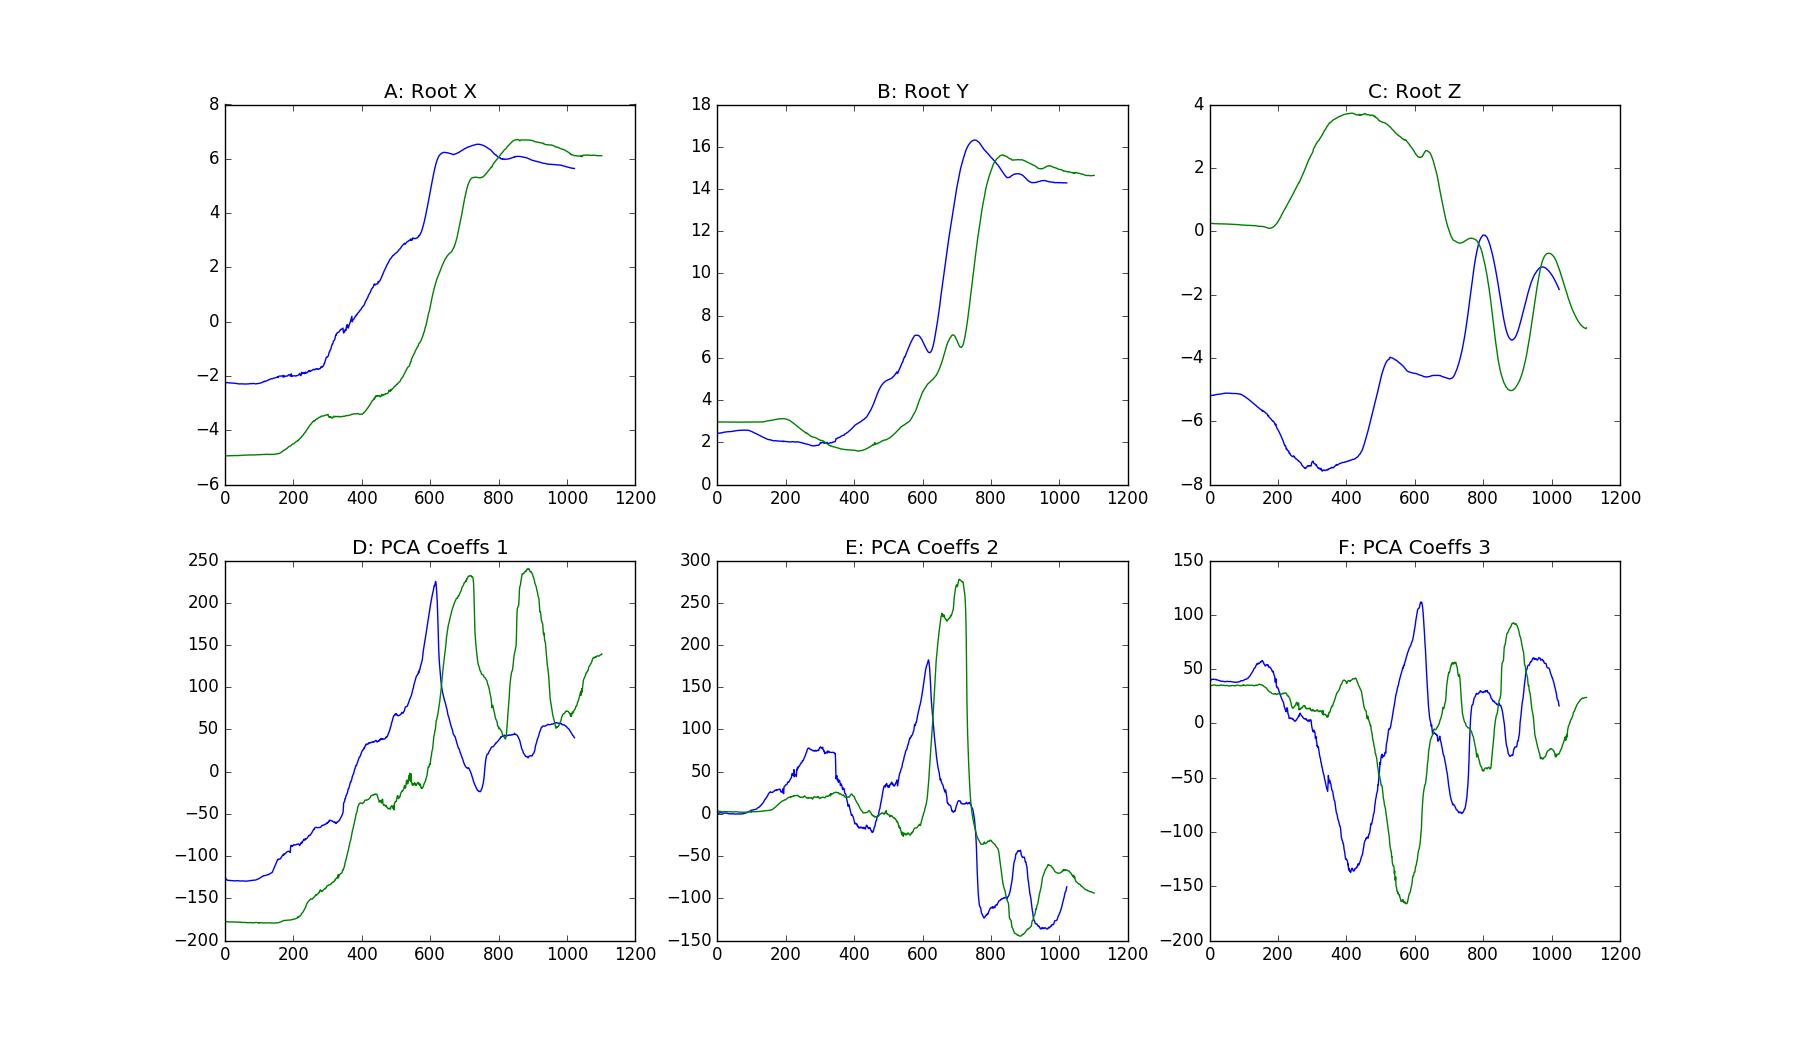
\includegraphics[width=\textwidth]{/home/cshome/j/jcampbell/Desktop/Thesis/Thesis/images/getting_up.png}
\caption{Motion capture data for a subject as they rise from the ground in two 	different examples. The top row shows the position of the root node of the subject while the bottom row shows the data projected according to the PCA basis functions, for each of the first three most significant components. In each of the plots the blue trace is for the first example while the green trace is for the second example. The same subject performed both actions. The two motion examples are 3 and 4 for subject 140 of the CMU Mocap database. \label{getting_up}}
\end{figure}

\begin{figure}[h]
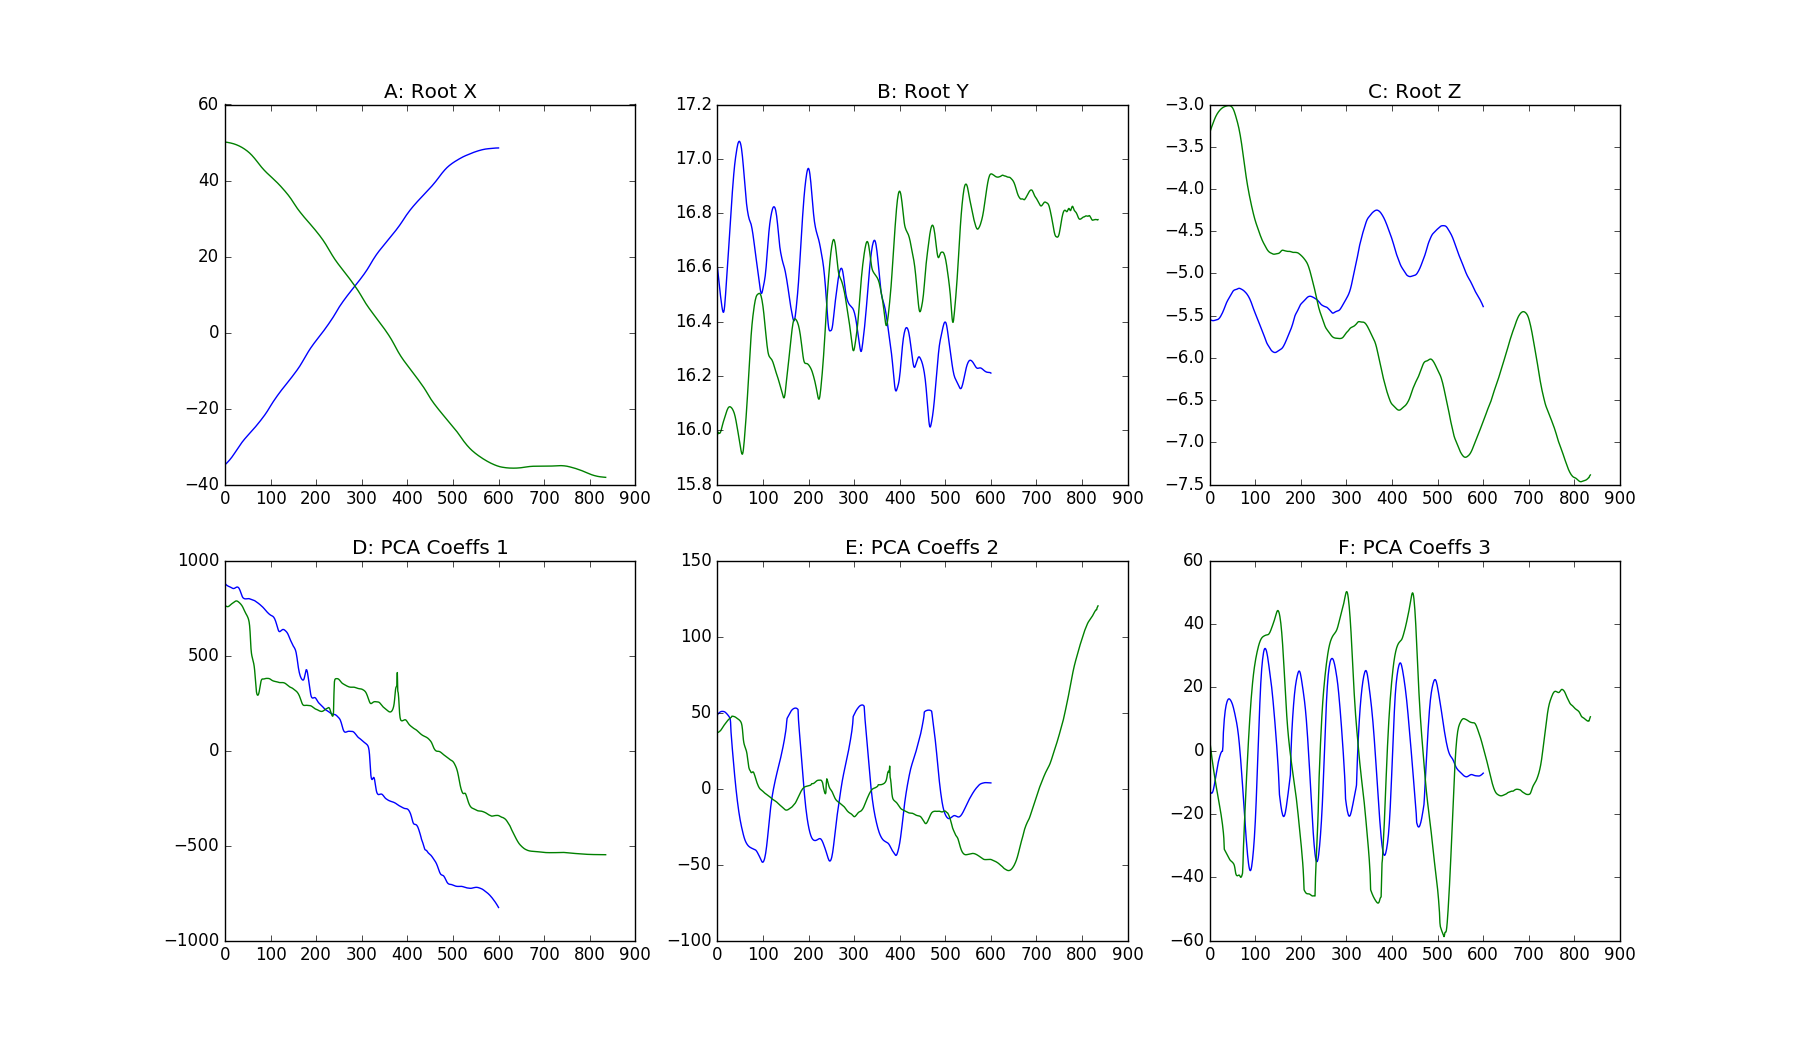
\includegraphics[width=\textwidth]{/home/cshome/j/jcampbell/Desktop/Thesis/Thesis/images/walks.png}
\caption{Motion capture data for a subject as they walk in two different examples. In both cases the subject walked for a short period in one direction and then turned and walked back. The top row shows the position of the root node of the subject while the bottom row shows the data projected according to the PCA basis functions, for each of the first three most significant components. In each of the plots the blue trace is for the first example while the green trace is for the second example. The same subject performed both actions. The two motion examples are 21 and 22 for subject 136 of the CMU Mocap database. \label{walks}}
\end{figure}

\subsection{Principle Component Analysis}

Principle component analysis (PCA) is a widely used method for computing a low dimensional representation of data. Given an $n\:\:\text{x}\:\:m$ data matrix $X$, PCA finds a linear transformation to a new set of coordinate axes such that the variance along each of the new axes is maximised. Typically singular value decomposition (SVD) is used to find this transformation. The PCA transform using SVD performs a factorisation of the data matrix according to

\begin{equation}
X = U \Sigma V^{T} 
\end{equation}

\noindent where $U$ and $V$ are the left and right singular vector matrices of size $n\:\:\text{x}\:\:n$ and $m\:\:\text{x}\:\:m$ respectively. The matrix $\Sigma$ is an $n\:\:\text{x}\:\:n$ diagonal matrix containing the $n$ singular values of $X$. The vectors of $V$ are eigenvectors of the covariance matrix $X X^{T}$ and represent the principle components of the transformed data. We transformed data matrix is found by projecting the original data matrix into the space defined by the PCA axes according to

\begin{equation}
Y = V X. 
\label{PCA_compute}
\end{equation}

This method, however, only works efficiently in cases where the dimensionality of each sample is much lower than the number of samples available, i.e. when $n > p$. This is because the covariance matrix $X X^{T}$ becomes very large. \\

It is often the case where the dimensionality of our samples is much greater than the number of samples available. We will see in later sections that this is the case for temporal synchronisation of videos. If we represent each frame of a video as a single vector then the dimensionality of each sample is equal to the number of pixels in the image. If our video is only 100 - 200 frames long, then we clearly have $p >> n$. In this situation we turn to an alternative method for estimating the principle components, as defined by reference. \\

Since the number of samples is low we can efficiently compute the alternative covariance matrix $X^{T} X$ which is of size $n\:\:\text{x}\:\:n$. We then compute the eigenvalues and eigenvectors of this covariance matrix. The matrix $V$ is formed by stacking the eigenvectors in columns according to the size of the corresponding eigenvalues and can then be used as in Eq. \ref{PCA_compute}.\\

\section{Synthetic Function Matching with HSIC}

The principle contribution of this section is to demonstrate that our HSIC based measure provides a robust measure of the similarity between two arbitrary time-series signals. We demonstrate this capability with a series of examples on synthetic data. As a further proof of concept we also demonstrate that our measure could be used to re-construct a signal from data, in cases where Fourier based methods are not suitable. \\

We saw in Figs \ref{getting_up} and \ref{walks} that our input is a multi-dimensional time-series signal. The top rows of each of these figures are raw input data, while the bottom rows are the PCA transformed data. In each plot we have traced a single parameter from each of two motions. Our input is given by the variables $X = \{x_0, x_1, ..., x_n\}$ and $Y = \{y_0, y_1, ..., y_n\}$, where each of the $n$ samples $x_i$ and $y_i$ are vectors of length $m$. Each element $x_{ik}$ and $y_{ik}$ of $x_i$ and $y_i$ gives the value of a single parameter at a single point in time. It may be, for example, that $x_i$ and $y_i$ are pixel intensities, spatial coordinates of a point on a moving target, or joint angles from motion capture data. As usual we have that $\text{HSIC}(X, Y) = \frac{1}{n^2}\text{tr}\textbf{(KHLH)}$ where $\textbf{H}$ is a centering matrix and $\textbf{K}$ and $\textbf{L}$ are Gram matrices defined on $X$ an $Y$ respectively. As before, our kernel matrix is defined as

\begin{equation}
\textbf{K}_{i,j} = k(x_i,y_j) = \exp^{-((x_i-y_j)\Sigma(x_i-y_j)^T)}
\end{equation}

\noindent where $\Sigma$ is a covariance matrix.\\

Before we begin a discussion of further experiments we first introduce our normalised version of the HSIC, which we term NHSIC. The NHSIC is defined as 

\begin{equation}
\text{NHSIC}(X,Y) = \frac{\text{HSIC}(X,Y)}{\sqrt{\text{HSIC}(X,X)\text{HSIC}(Y,Y)}}
\end{equation}

\noindent and is necessary because, as we will see, we need to vary the choice of (co)-variance for any choice of $X$ and $Y$. We therefore need to scale the HSIC value in order to be able to compare any two results. This will be elaborated further below. \\

In previous works a number of authors have used the median of the data values as the variance in the kernel function. We show instead that it is better to estimate the (co)-variance from the data. This produces much more stable results than the median value, which is important if we are using the NHSIC as an energy measure in an optimisation schema. In Fig. \ref{var_med} we show how the choice of variance affects the HSIC between a fixed signal and a signal with a varying amplitude. In the left plot we can see that the NHSIC varies smoothly with changes in the amplitude of the test signal, while in the right plot the NHSIC results are noisy and contain a significant number of local minima.\\

\begin{figure}[h]
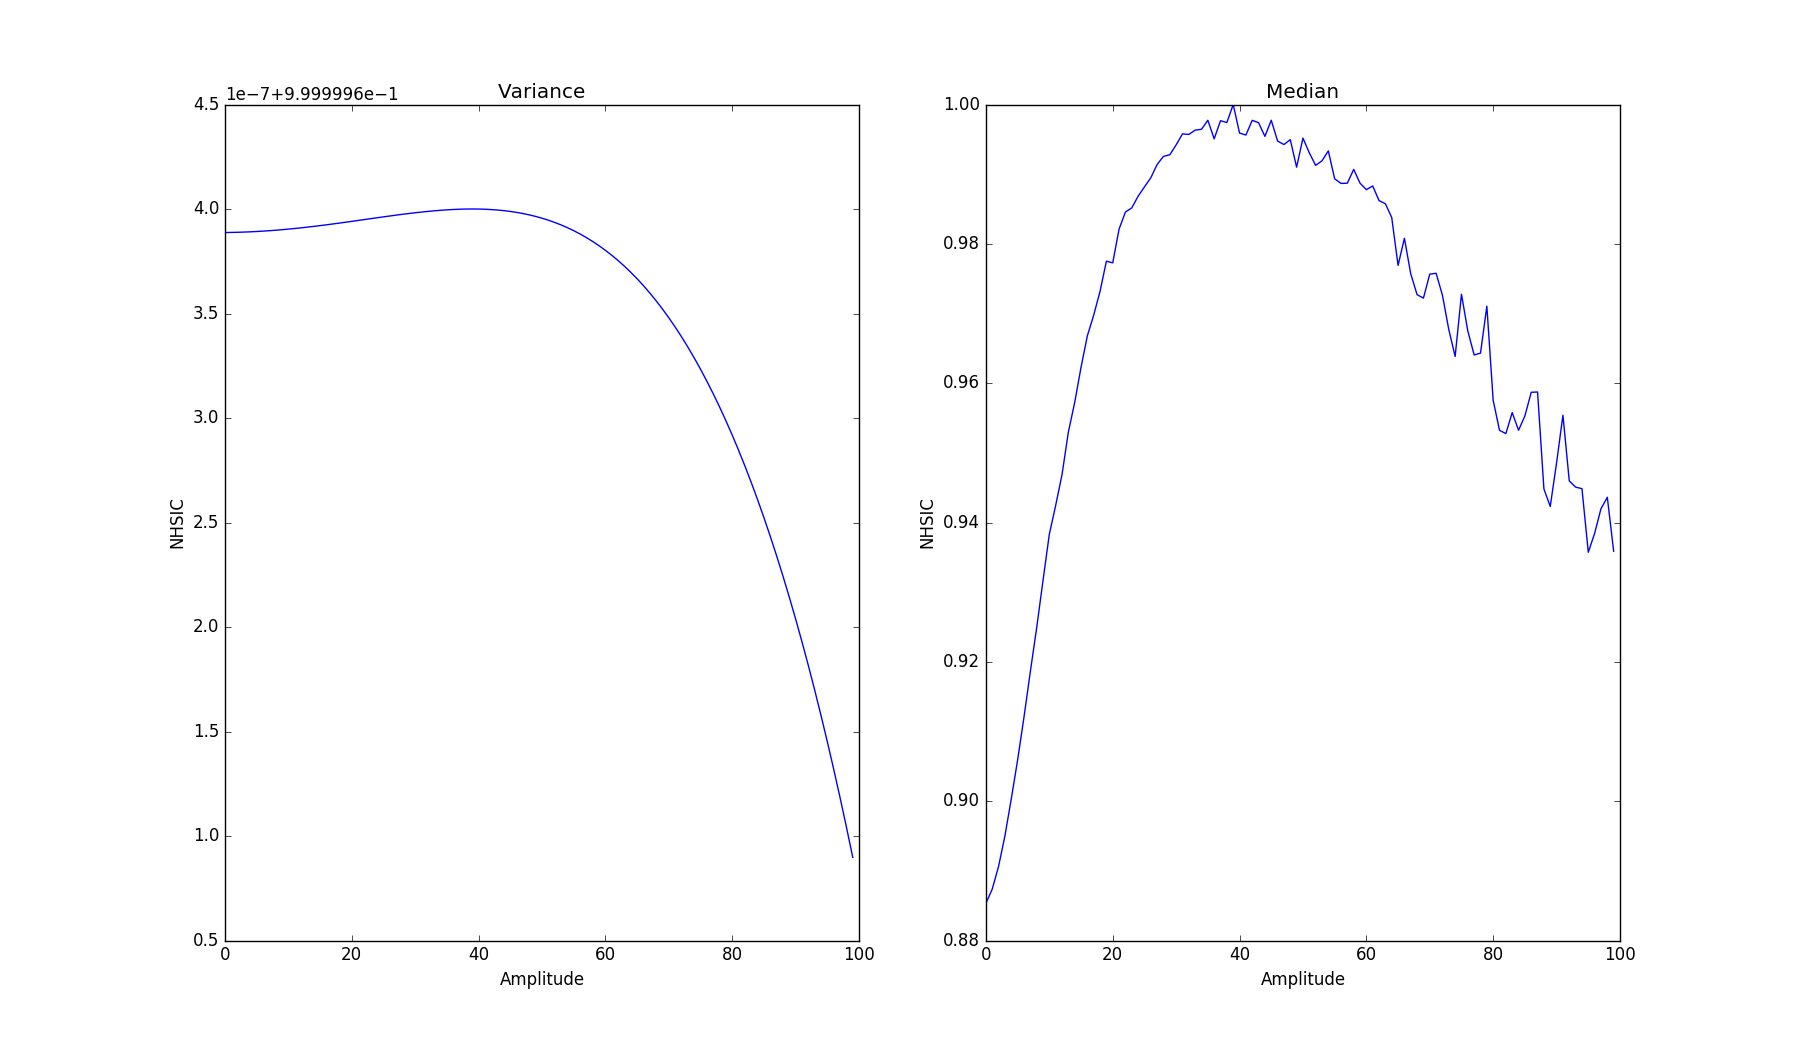
\includegraphics[width=\textwidth]{/home/cshome/j/jcampbell/Desktop/Thesis/Thesis/images/var_med.png}
\caption{NHSIC results using the variance estimated from data (left plot) and the median of the values (right plot) to measure the similarity between a signal with a fixed amplitude and another with a varying amplitude. It is difficult to see in the left plot however the maximum value 9at index 39) is correct, as is that for the right plot.  \label{var_med}}
\end{figure}

One of the consequences of performing computations on sine waves is that the variance of the signal increases quadratically with linear increases in the amplitude. This effect can be seen in Fig. \ref{amp_var} which demonstrates the changes in variance as the amplitude of a sine wave increases. If we were to choose a fixed value for the (co)-variance in the kernel function, then we would effectively be restricting the domain of the kernel function given the variance of the input signal. At first glance this would seem fine, as it is our goal to discover differences in two signals, which will clearly be uncovered if our kernel function treats signals with different variances differently. The problem, however, is that as the magnitude of a sine wave approaches infinity, the HSIC will approach a value of one. This means that a signal with a large amplitude is deemed more similar to a reference signal than the reference signal with itself. If we are given the three functions: $f_1(x) = 0.9\sin(x)$, $f_2(x) = 0.25\sin(x)$, and $f_3(x) = 2.5\sin(x)$, with the goal of asking which of $f_1$, $f_1$, or $f_1$ is most similar to $f_{\text{ref}}(x) = \sin(x)$, then we would be given $f_3$ as the closest match. Notably, if the (co)-variance of the kernel function is fixed, then we would have that $\text{HSIC}(f_{\text{ref}}, f_3) > \text{HSIC}(f_{\text{ref}}, f_{\text{ref}})$. Thankfully the solution to this problem is very simple: we require only that the variance of the kernel function be estimated independently for any HSIC computation. As mentioned previously, however, this means that we must also normalise the resulting HSIC value.  \\

In Figs. \ref{fixed_var_no_norm}, \ref{floating_var_no_norm}, \ref{fixed_var_normalisation}, and \ref{floating_var_normalisation} we show the effect of computing the HSIC between two sine waves, one with varying amplitude and frequency, under a number of different conditions. In all four of these experiments the same test sine wave was used. In Figs. \ref{fixed_var_no_norm} and \ref{floating_var_no_norm} the incorrect result is returned, while in Fig. \ref{fixed_var_normalisation} the correct result is returned, however it is less distinct than the (correct) results in Fig. \ref{floating_var_normalisation}. It is difficult to see in these examples, however the correct frequency is obtained for almost all magnitudes. In Fig. \ref{freq} we can see that at the correct magnitude the correct frequency is clearly found by our algorithm. 



\begin{figure}[h]
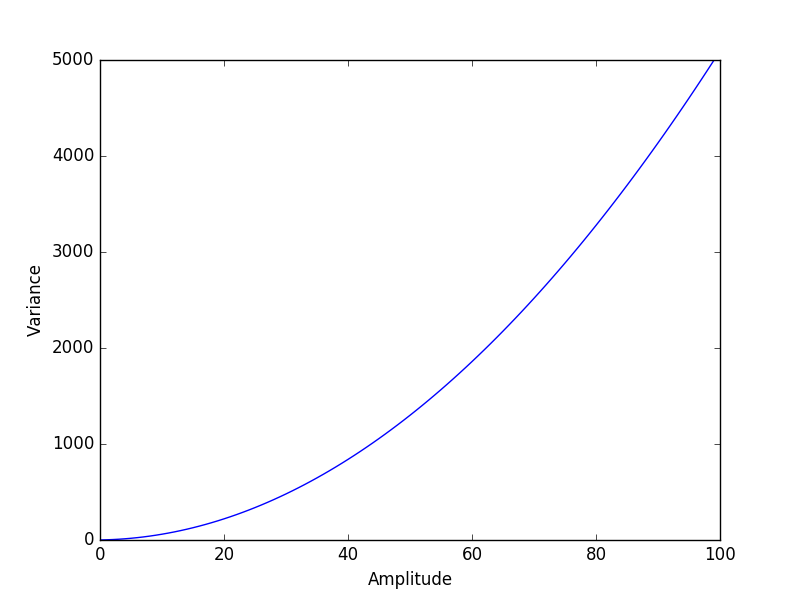
\includegraphics[width=\textwidth]{/home/cshome/j/jcampbell/Desktop/Thesis/Thesis/images/amp_var.png}
\caption{Variance of a sine wave as the amplitude is linearly increased.\label{amp_var}}
\end{figure}

\begin{figure}[h]
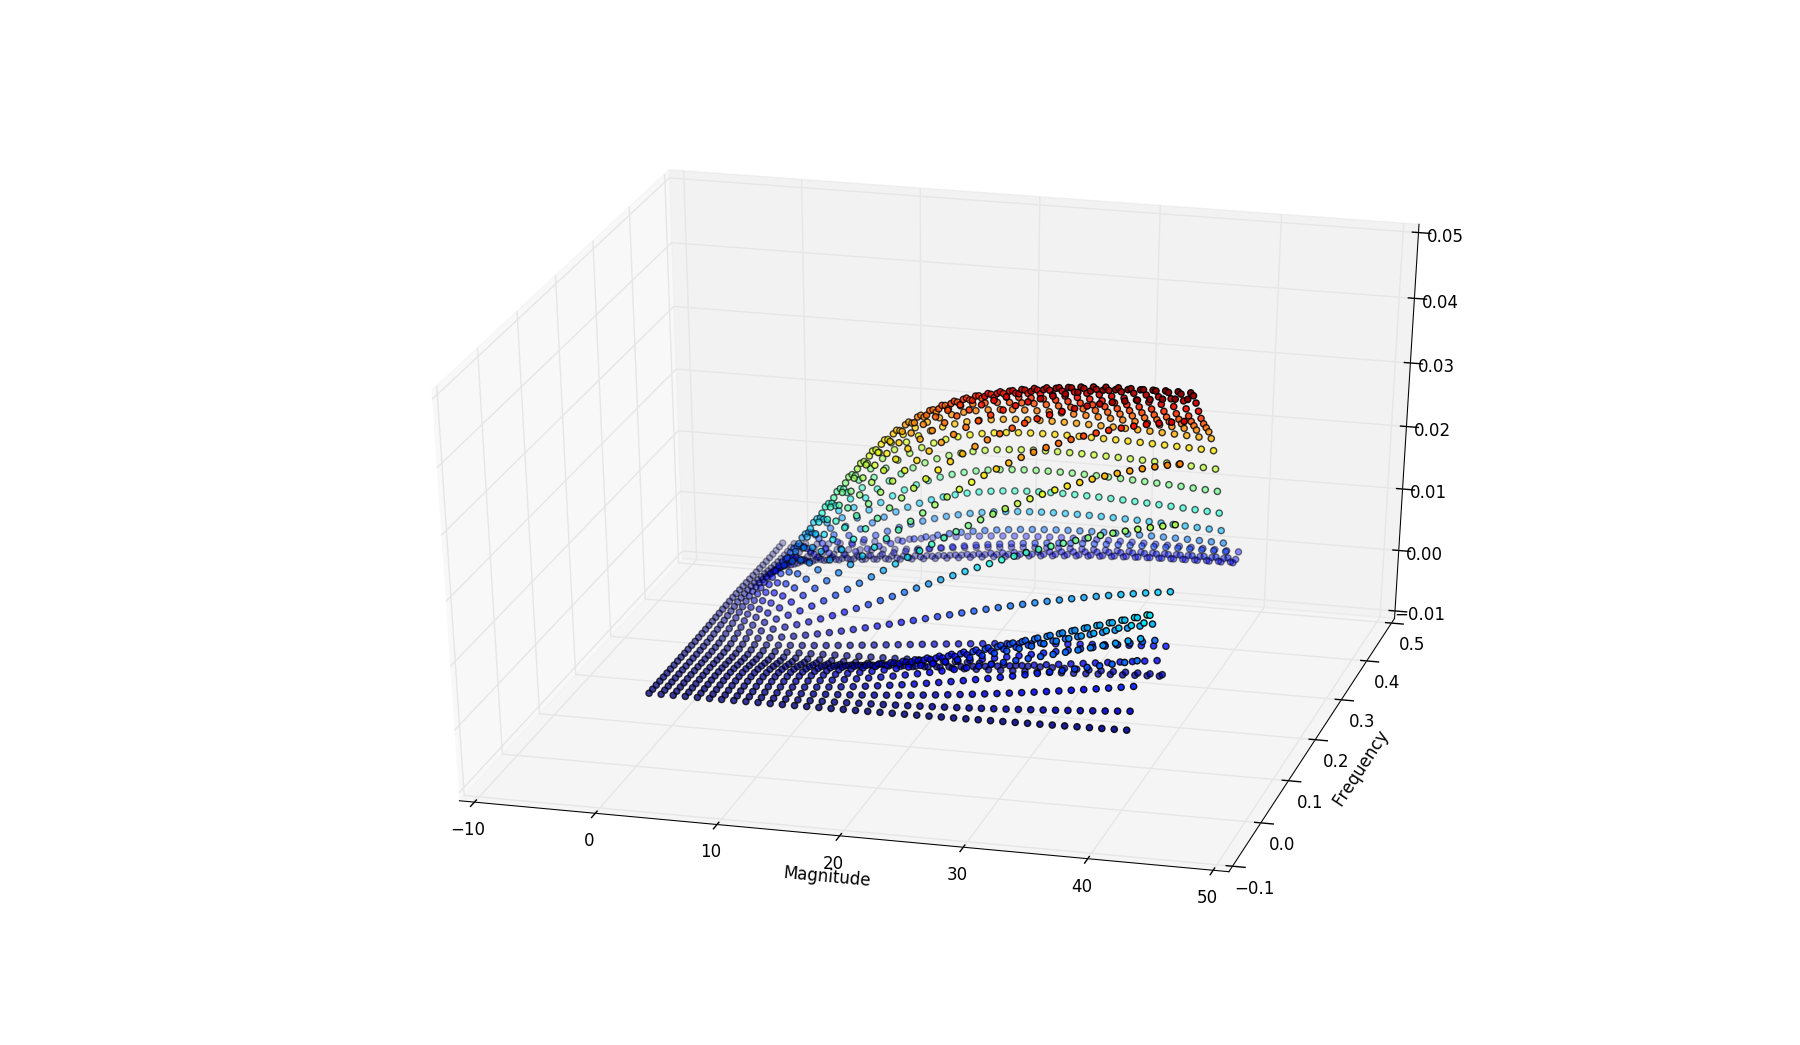
\includegraphics[width=\textwidth]{/home/cshome/j/jcampbell/Desktop/Thesis/Thesis/images/fixed_var_no_norm.png}
\caption{Variance computed from all possible examples, with no normalisation of the HSIC. Note that the peak is pronounced, however it incorrectly identifies the magnitude. \label{fixed_var_no_norm}}
\end{figure}

\begin{figure}[h]
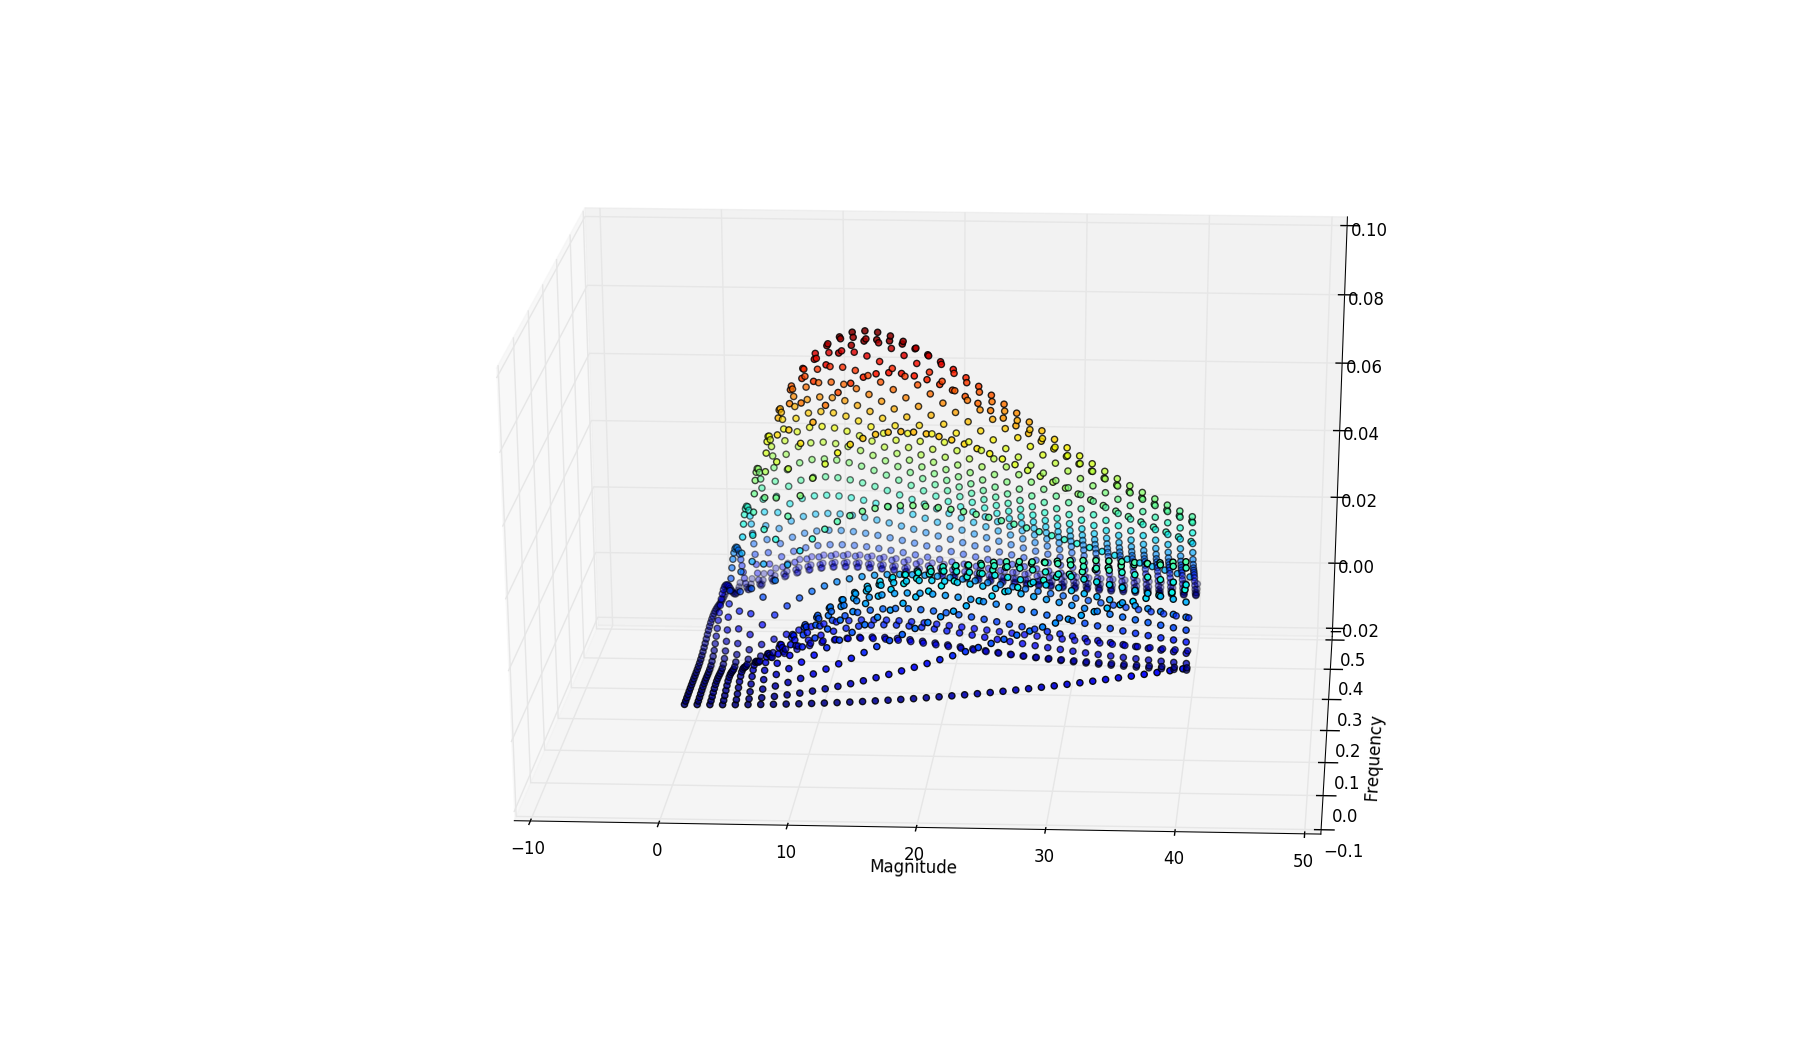
\includegraphics[width=\textwidth]{/home/cshome/j/jcampbell/Desktop/Thesis/Thesis/images/floating_var_no_norm.png}
\caption{Variance computed independently for every test example, with no normalisation of the HSIC. The peak is\label{floating_var_no_norm}}
\end{figure}

\begin{figure}[h]
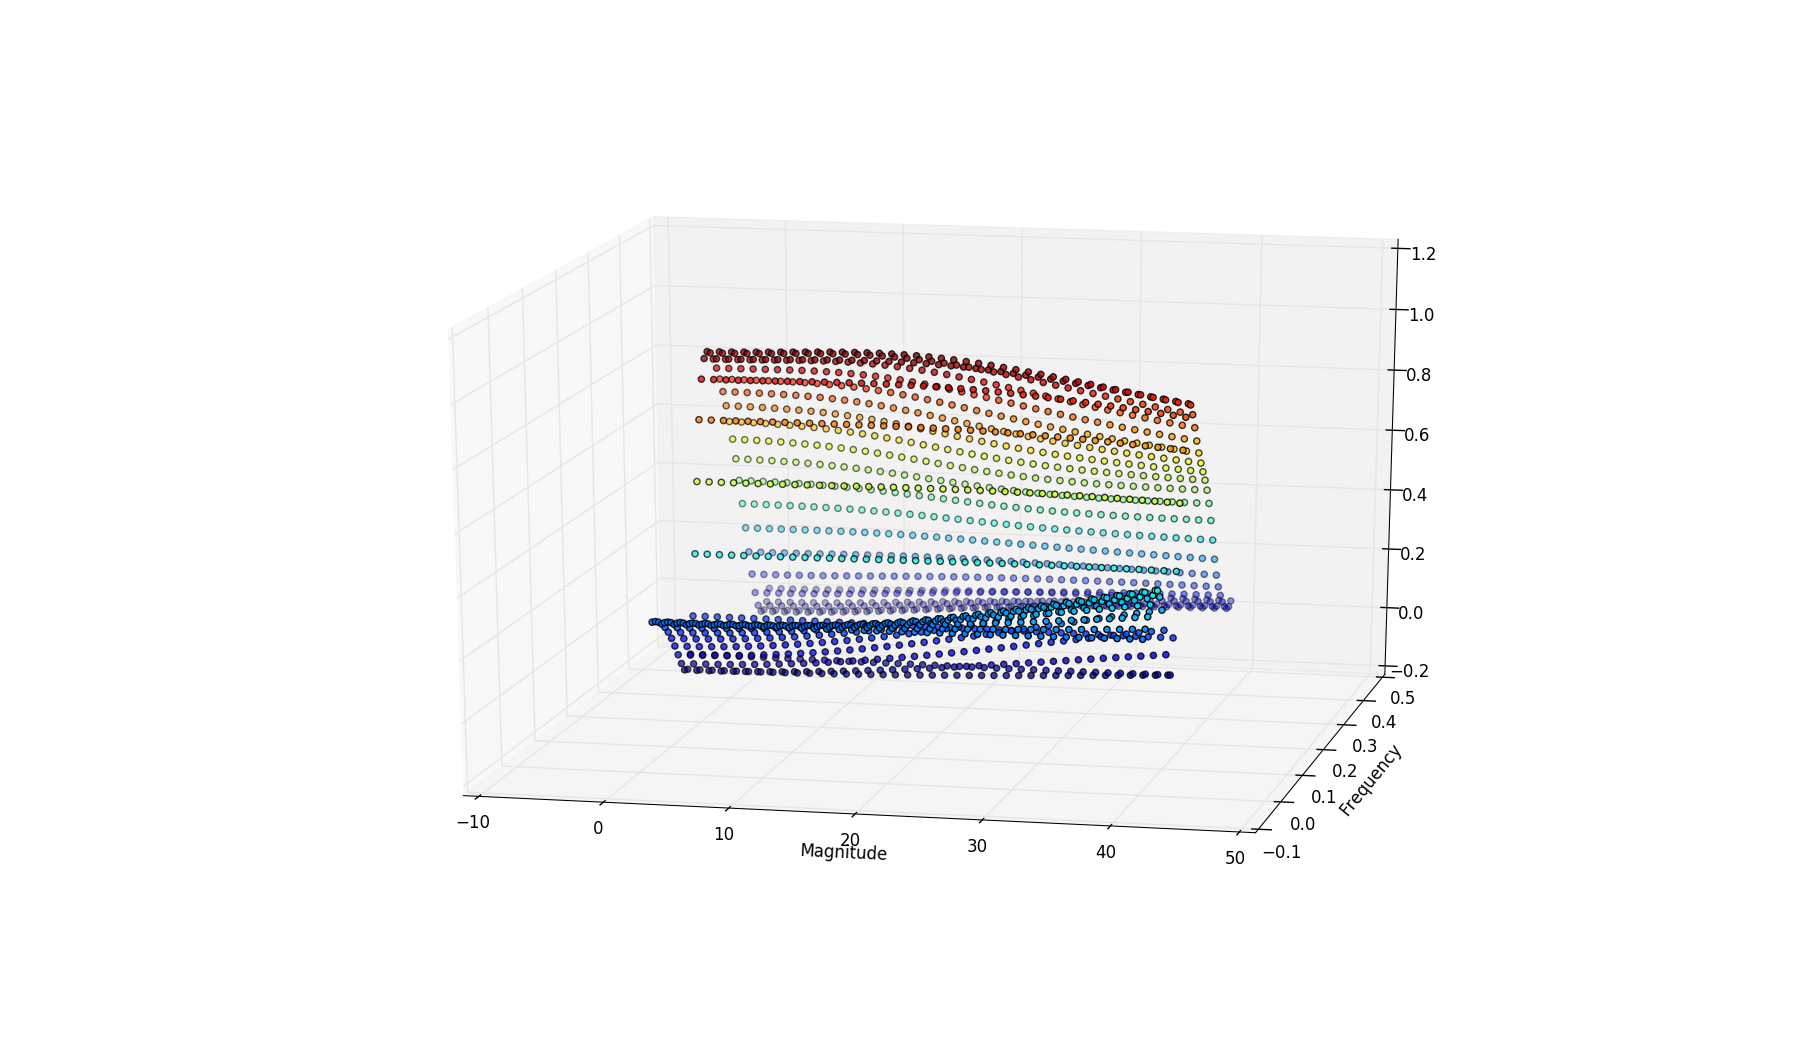
\includegraphics[width=\textwidth]{/home/cshome/j/jcampbell/Desktop/Thesis/Thesis/images/fixed_var_normalisation.png}
\caption{Variance computed from all possible examples, with normalisation of the HSIC.\label{fixed_var_normalisation}}
\end{figure}

\begin{figure}[h]
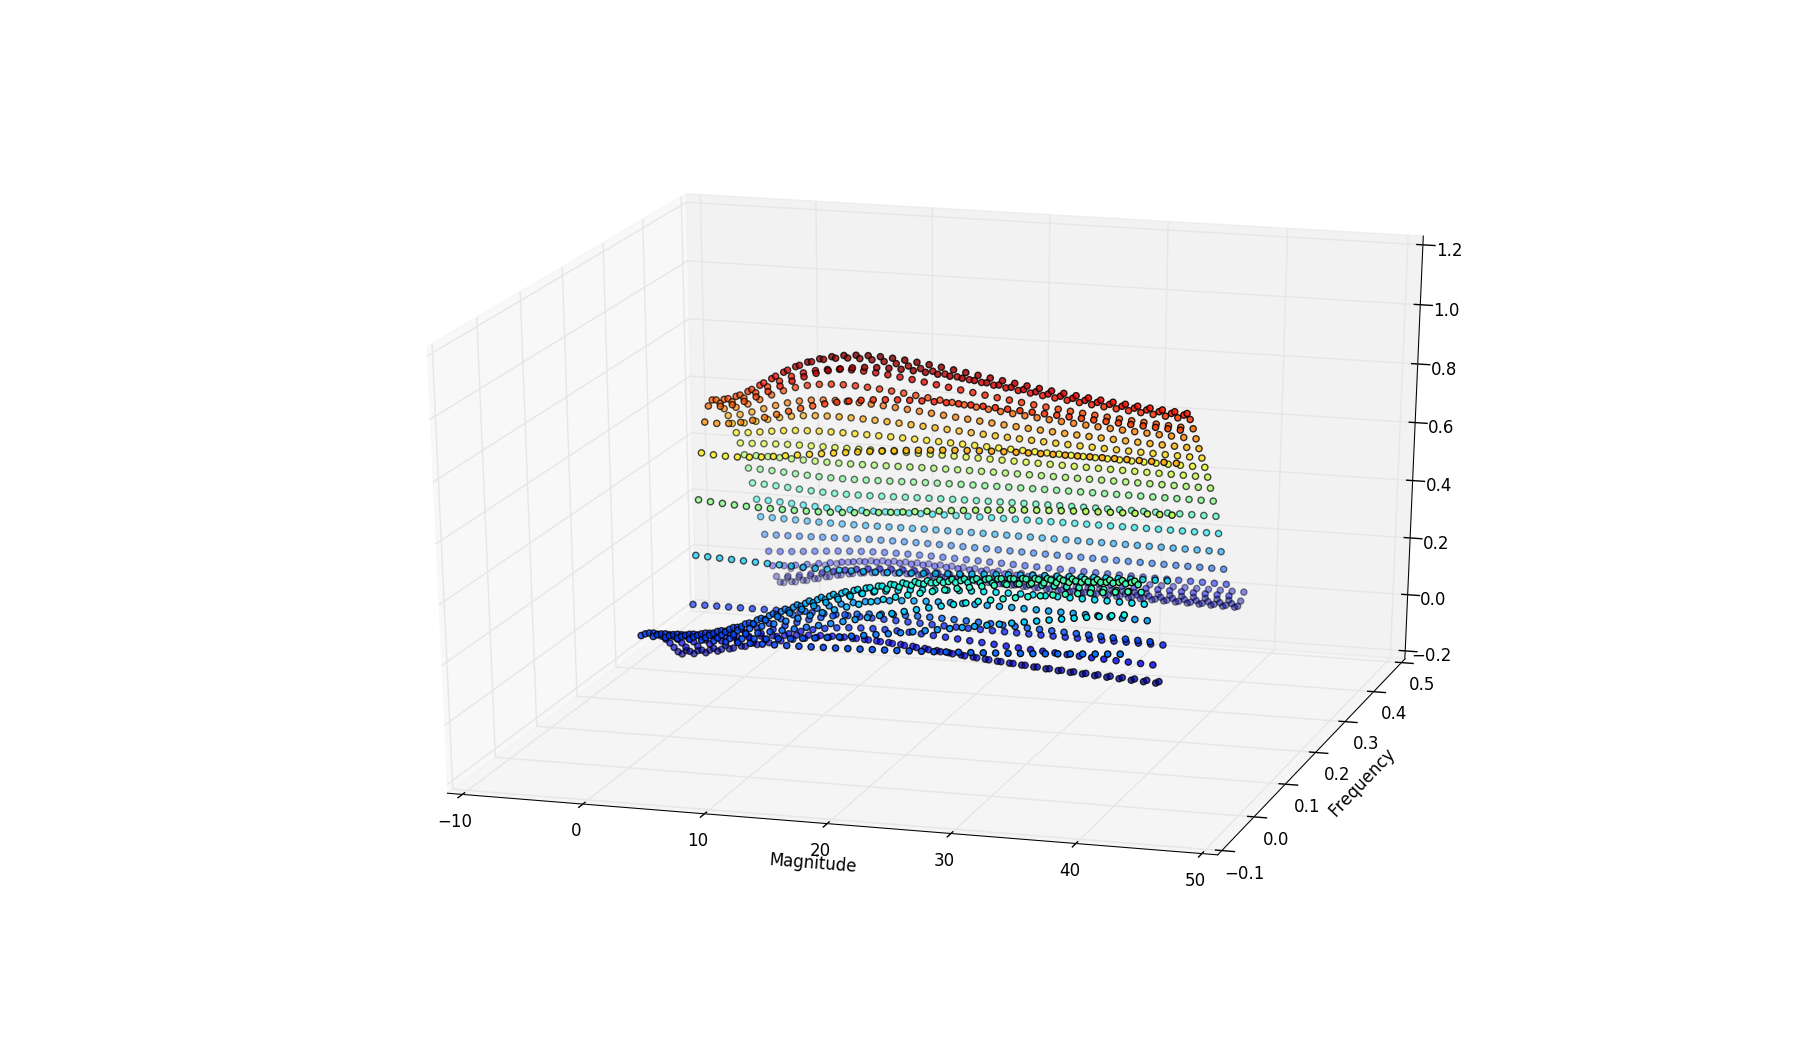
\includegraphics[width=\textwidth]{/home/cshome/j/jcampbell/Desktop/Thesis/Thesis/images/floating_var_normalisation.png}
\caption{\label{floating_var_normalisation}}
\end{figure}

\begin{figure}[h]
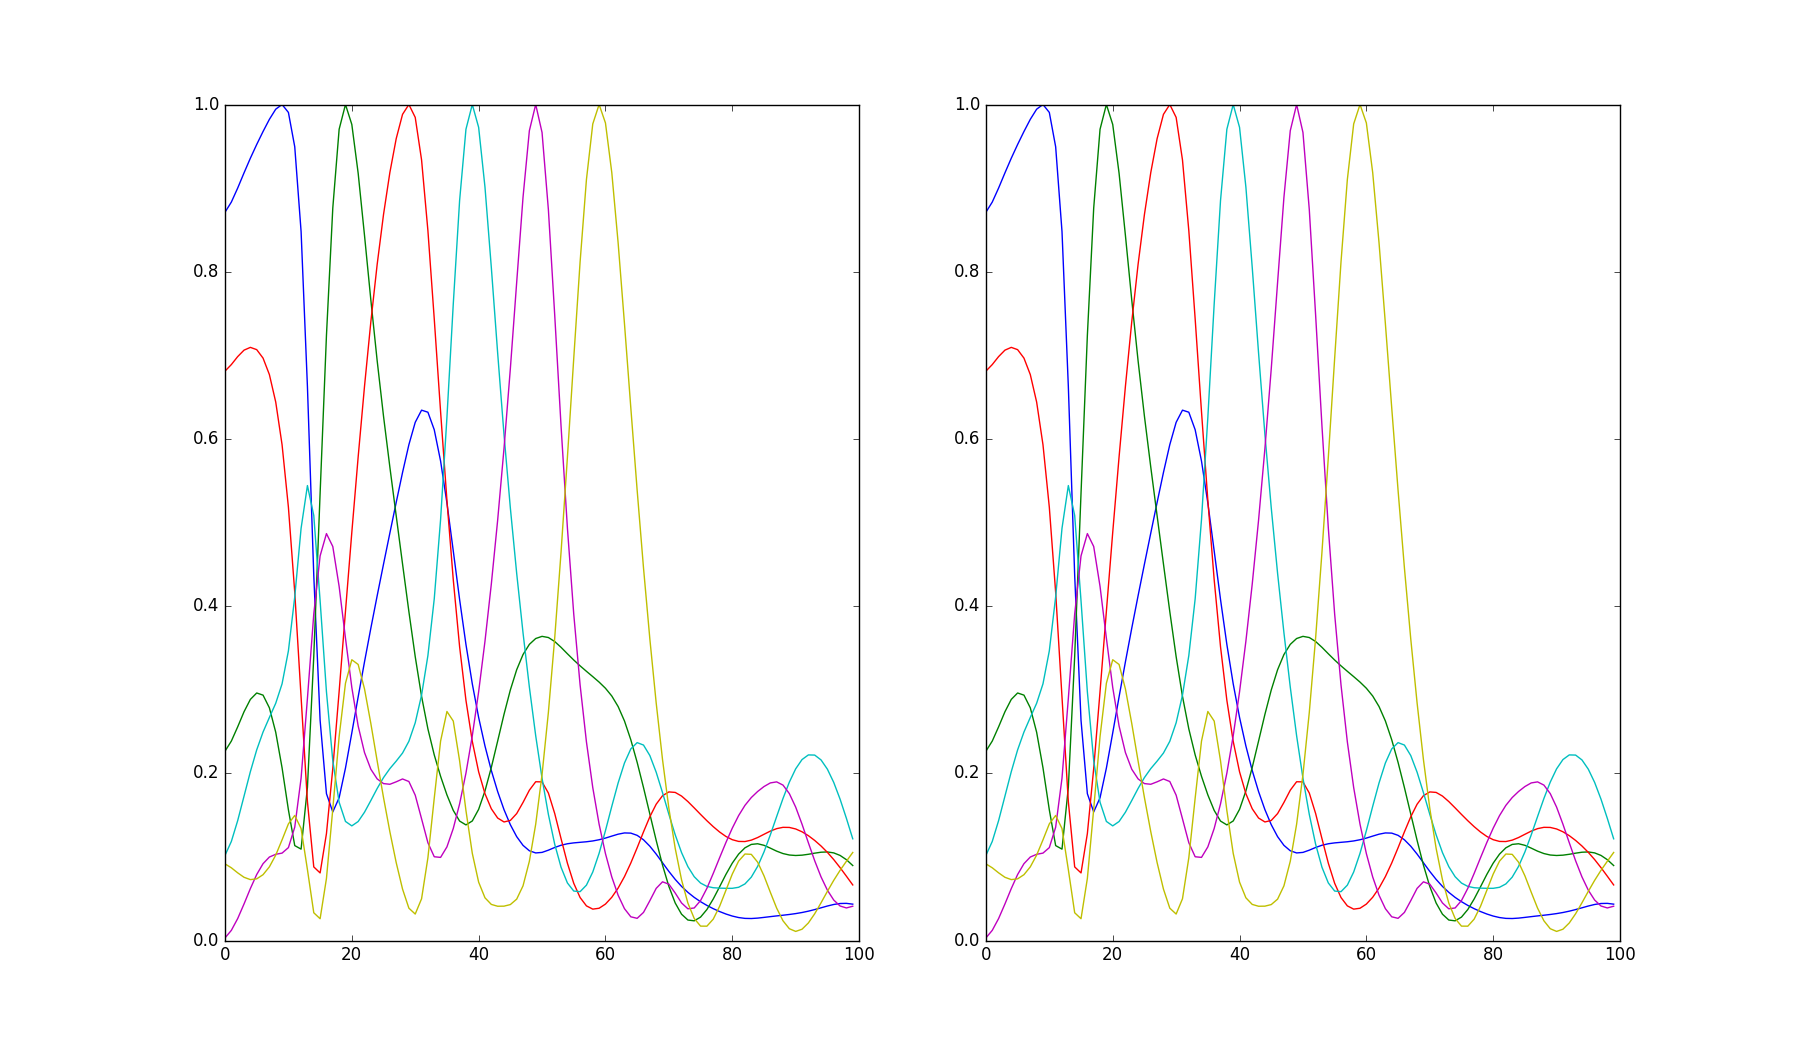
\includegraphics[width=\textwidth]{/home/cshome/j/jcampbell/Desktop/Thesis/Thesis/images/freq.png}
\caption{\label{freq}}
\end{figure}

\begin{figure}[h]
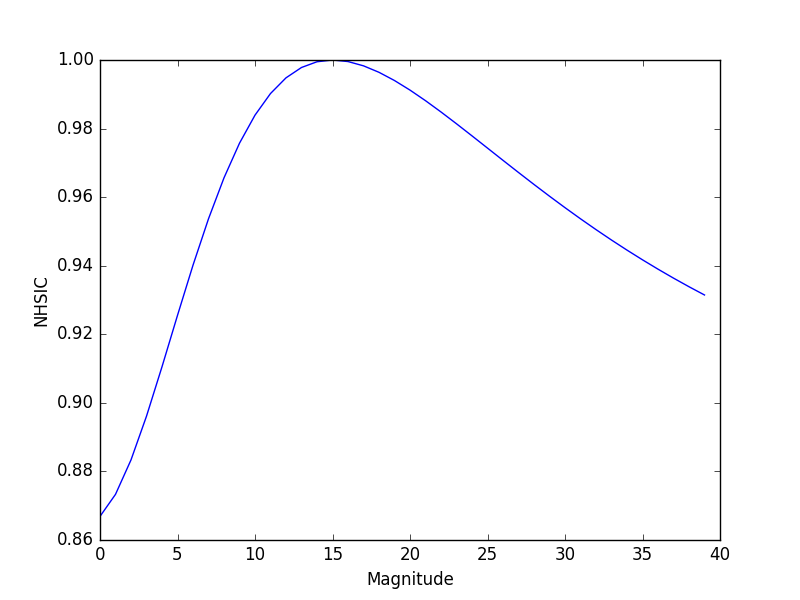
\includegraphics[width=\textwidth]{/home/cshome/j/jcampbell/Desktop/Thesis/Thesis/images/magnitude.png}
\caption{\label{magnitude}}
\end{figure}































\section{Action Recognition}

We turn now to the principle contribution of this chapter: to demonstrate that the Hilbert-Schmidt independence criterion can be used to match sequences of activities from motion capture data. As before we use the normalised HSIC, and estimate the covariance of the data for every pair of activities we wish to match. \\%One of the limitations of our method is that for any two action sequences we compare, we require that they are of equal length. We cannot match, for instance, a four second video of a person walking with an eight second video of a person walking.  This is less of a problem in cases where we are searching for instances of a reference action in a longer sequence, however we must account for the length of the input when matching two sequences in their entirety. This will be further discussed in section something.\\

In our first experiments we are given a short reference sequence of a walking motion, along with a longer video that contains various examples of both walking and climbing behaviour. The PCA transformed reference input is $X = \{x_0, x_1, ..., x_N\}$ where each $x_i$ is a $Q$ dimensional vector containing the $Q$ most significant components. We choose the number of PCA components, $Q$, for each experiment according to 

\begin{equation}
z = \frac{\sum_k^Q{\sqrt{e_k}}}{\sum_i^N{\sqrt{e_i}}} > 0.95
\end{equation}

\noindent where $e_i$ is the i\textit{th} eigenvalue of the principle components and $N$ is the number of samples. This allows us to choose the smallest number of principle components that explain more than $95\%$ of the variance of the data.\\

\begin{figure}[h]
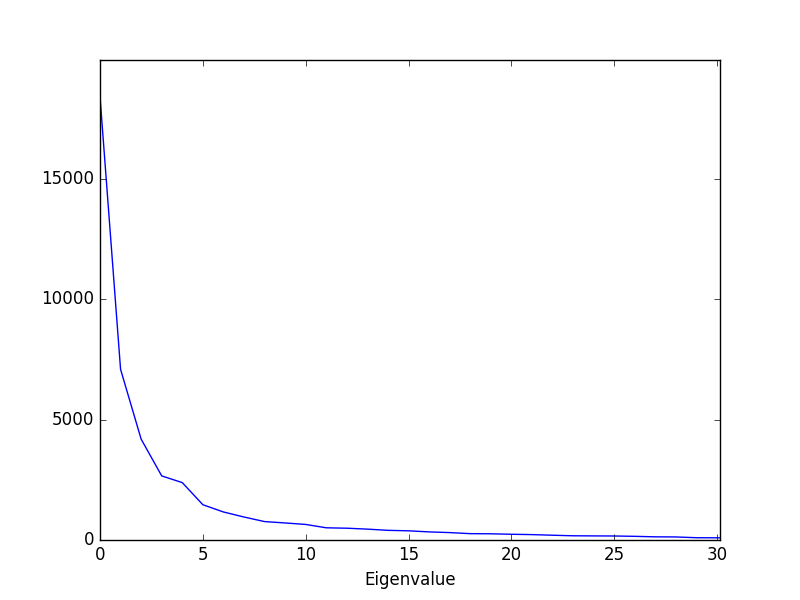
\includegraphics[width=\textwidth]{/home/cshome/j/jcampbell/Desktop/Thesis/Thesis/images/eigenvalues.png}
\caption{Plot of the square root of the eigenvalues of the data covariance matrix, in decreasing order. Only the first 30 values are shown for display purposes. \label{eigenvalues}}
\end{figure}

Our initial reference video is number 34 from subject 105 (herein referred to as 105/34) of the CMU Mocap database. Our test video is number two from subject one (herein referred to as 01/02) of the same database. In this experiment $Q$ is set to 29, as this is the larger of the $Q$ values for the two sequences. From 105/34 we selected a six second walking sequence as the reference motion, which corresponds to 720 mocap data samples. We use a number of reference sequences offset slightly from the starting point to reduce the sensitivity of our algorithm to changes in phase. Selected frames from the animated reference and test sequences are shown in Figs. \ref{105_34} and \ref{01_02} respectively. The frames in Fig. \ref{105_34} are indicative of all the subsequences used. The frames in Fig \ref{01_02} are from the closest matching subsequence from 01/02, i.e the subsequence that most resembles walking motion, according to our algorithm. Fig. \ref{ts_05} shows the results of running the NHSIC algorithm for a variety of offsets of the test sequence. Each sequence contains $M = 720$ data samples, however this is downsampled to $N = 200$ samples as the time complexity of the NHSIC algorithm has time complexity $O(N^2)$. There are two peaks in the results in Fig. \ref{ts_05}: at frame 45 and frame 104. The first peak correctly indicates the point in the sequence when the subject is walking, while the second peak refers to a subsequence for which the subject is climbing a set of stairs. These results are interesting as one would not typically not label a stair climbing sequence as walking, which raises an interesting problem with our algorithm: we currently have neither an objective measure of success, nor do we have any means of selecting against negative examples. These two problems are discussed after the presentation of the results. These results do, however, clearly demonstrates the strength of the Hilbert-Schmidt independence criterion to match sequences which share common underlying characteristics.% To further demonstrate the strength of the NHSIC, Fig. \ref{ts_09_expanded} shows an expanded section of results from Fig. \ref{ts_09}, which highlights the twin peaks at frames 105 and 108, with a much lower result at frame 107, between them. This drop corresponds to a subsequence where the subject climbs the stairs, waits, and then climbs back down. The peaks on either side of this drop refer to subsequences where the subject is predominantly climbing either up or down the stairs. \\

We further tested our algorithm with the same reference sequence (105/34) but with a different test sequence: video 15 from subject 86 (86/15) of the CMU mocap database. In this video the subject walks in a small circle for a short period of time, sits down, waves their arms, makes a number of miscellaneous actions, then stands and walks in a small circle again. The results of running our algorithm under the same conditions as the previous experiment are shown in Fig. \ref{ts_08}, where we can clearly see the strong match at the start of the sequence (frames 0 - 22), and at the end of the sequence (frame 210). These results also show a weaker match at frames 93 - 103. This weaker match occurs when the subject is sitting and makes a brushing motion with their arm. Since this motion is isolated (does not appear in conjunction with other motions) it is being labelled as similar to the reference walking motion. This highlights the issue with the NHSIC for identifying false positives and is discussed further in the future work section. \\

Our final experiment of this section was on sequence eight from subject 86 (86/08) of the CMU mocap database. This subject initially walks, then performs a series of squats, twists, cyclical arm motions, and kicks. The subject then runs for a short period of time before performing punching actions and then walking again. Our algorithm identified approximately four motions that closely resembled walking. Two of these are indeed walking motions, however it also identifies the running period and kicking period as walking. The walking periods were the two closest matches, followed by the running period and then the kicking action. 

\begin{figure}
\centering
\begin{subfigure}{0.24\textwidth}
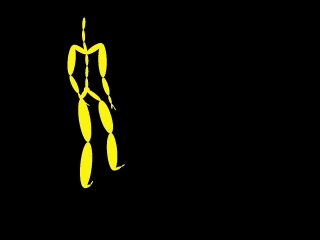
\includegraphics[width=\textwidth]{/home/cshome/j/jcampbell/Desktop/Thesis/Thesis/images/105_34/105.png}
\end{subfigure}
\begin{subfigure}{0.24\textwidth}

\includegraphics[width=\textwidth]{/home/cshome/j/jcampbell/Desktop/Thesis/Thesis/images/105_34/130.png}
\end{subfigure}
\begin{subfigure}{0.24\textwidth}
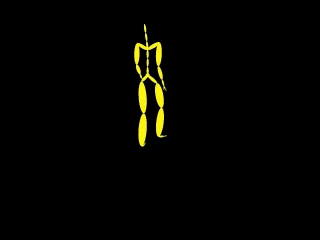
\includegraphics[width=\textwidth]{/home/cshome/j/jcampbell/Desktop/Thesis/Thesis/images/105_34/155.png}
\end{subfigure}
\begin{subfigure}{0.24\textwidth}
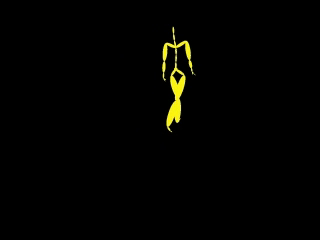
\includegraphics[width=\textwidth]{/home/cshome/j/jcampbell/Desktop/Thesis/Thesis/images/105_34/180.png}
\end{subfigure}

\begin{subfigure}{0.24\textwidth}
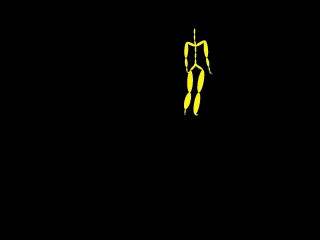
\includegraphics[width=\textwidth]{/home/cshome/j/jcampbell/Desktop/Thesis/Thesis/images/105_34/205.png}
\end{subfigure}
\begin{subfigure}{0.24\textwidth}
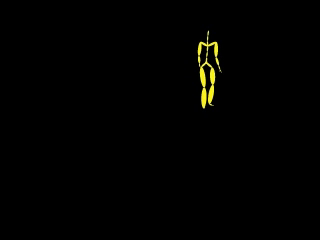
\includegraphics[width=\textwidth]{/home/cshome/j/jcampbell/Desktop/Thesis/Thesis/images/105_34/230.png}
\end{subfigure}
\begin{subfigure}{0.24\textwidth}
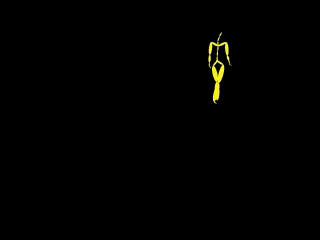
\includegraphics[width=\textwidth]{/home/cshome/j/jcampbell/Desktop/Thesis/Thesis/images/105_34/255.png}
\end{subfigure}
\begin{subfigure}{0.24\textwidth}
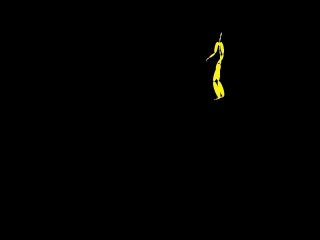
\includegraphics[width=\textwidth]{/home/cshome/j/jcampbell/Desktop/Thesis/Thesis/images/105_34/285.png}
\end{subfigure}
\caption{ Selected frames from the reference sequence of 105/34.   \label{105_34}}
\end{figure}

\begin{figure}
\centering
\begin{subfigure}{0.24\textwidth}
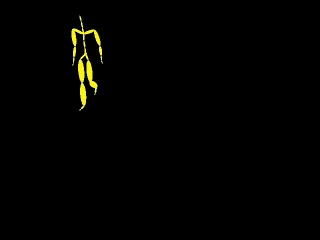
\includegraphics[width=\textwidth]{/home/cshome/j/jcampbell/Desktop/Thesis/Thesis/images/01_02/335.png}
\end{subfigure}
\begin{subfigure}{0.24\textwidth}
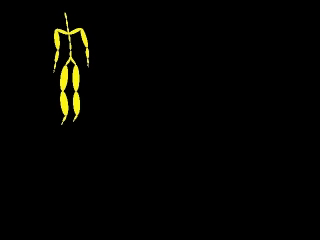
\includegraphics[width=\textwidth]{/home/cshome/j/jcampbell/Desktop/Thesis/Thesis/images/01_02/360.png}
\end{subfigure}
\begin{subfigure}{0.24\textwidth}
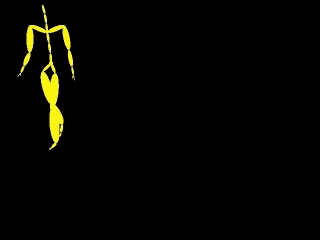
\includegraphics[width=\textwidth]{/home/cshome/j/jcampbell/Desktop/Thesis/Thesis/images/01_02/385.png}
\end{subfigure}
\begin{subfigure}{0.24\textwidth}
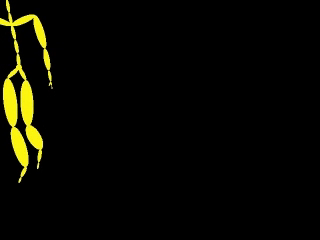
\includegraphics[width=\textwidth]{/home/cshome/j/jcampbell/Desktop/Thesis/Thesis/images/01_02/410.png}
\end{subfigure}

\begin{subfigure}{0.24\textwidth}
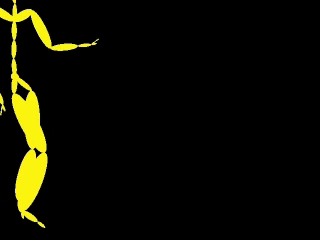
\includegraphics[width=\textwidth]{/home/cshome/j/jcampbell/Desktop/Thesis/Thesis/images/01_02/435.png}
\end{subfigure}
\begin{subfigure}{0.24\textwidth}
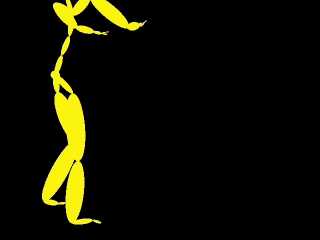
\includegraphics[width=\textwidth]{/home/cshome/j/jcampbell/Desktop/Thesis/Thesis/images/01_02/460.png}
\end{subfigure}
\begin{subfigure}{0.24\textwidth}
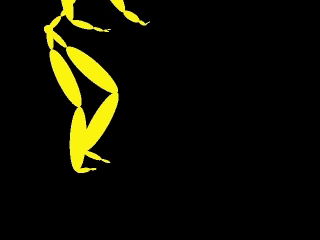
\includegraphics[width=\textwidth]{/home/cshome/j/jcampbell/Desktop/Thesis/Thesis/images/01_02/485.png}
\end{subfigure}
\begin{subfigure}{0.24\textwidth}
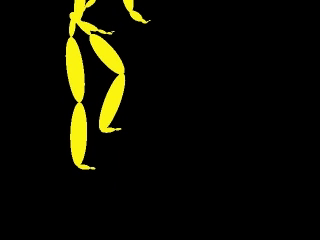
\includegraphics[width=\textwidth]{/home/cshome/j/jcampbell/Desktop/Thesis/Thesis/images/01_02/500.png}
\end{subfigure}
\caption{Selected frames from the subsequence of 01/02 that matches the reference sequence in 105/34.\label{01_02}}
\end{figure}

\begin{figure}[h]
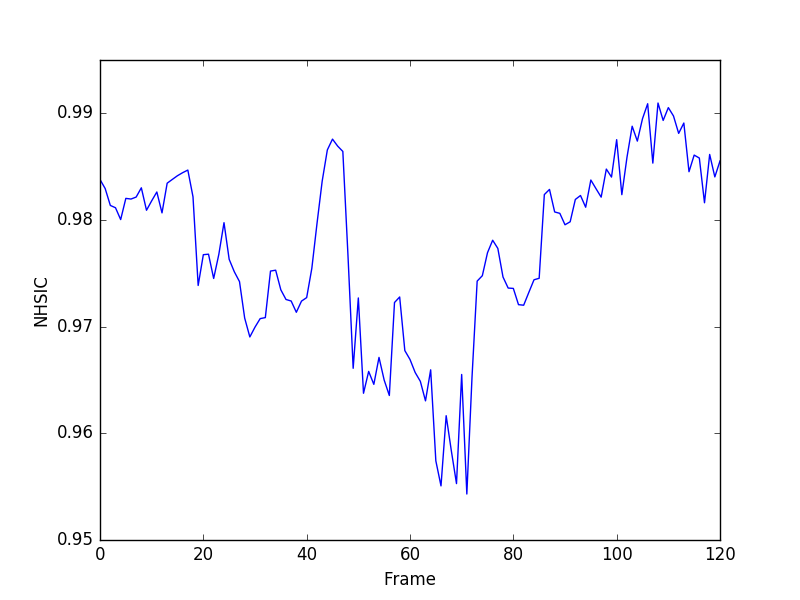
\includegraphics[width=\textwidth]{/home/cshome/j/jcampbell/Desktop/Thesis/Thesis/images/ts_09.png}
\caption{Activity recognition results for 01/02. Note the strong peak at frame 45 (walking) and the broader peak at frames 104 - 112 (climbing stairs).\label{ts_09}}
\end{figure}

%\begin{figure}[h]
%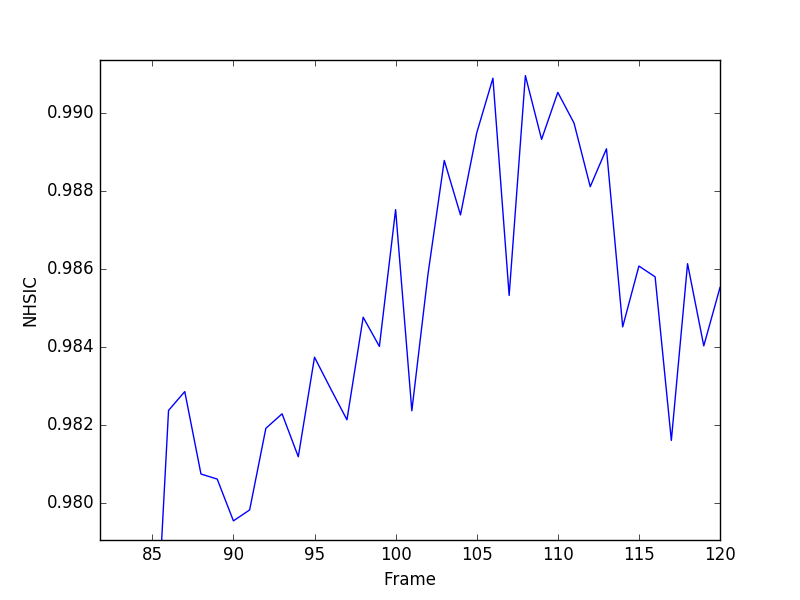
\includegraphics[width=\textwidth]{/home/cshome/j/jcampbell/Desktop/Thesis/Thesis/images/ts_09_expanded.png}
%\caption{Expanded results from Fig. \ref{ts_09} for frames 85 - 120. The subject begins climbing the stairs at frame 104, reaches the top at frame  \label{ts_09_expanded}}
%\end{figure}

\begin{figure}[h]
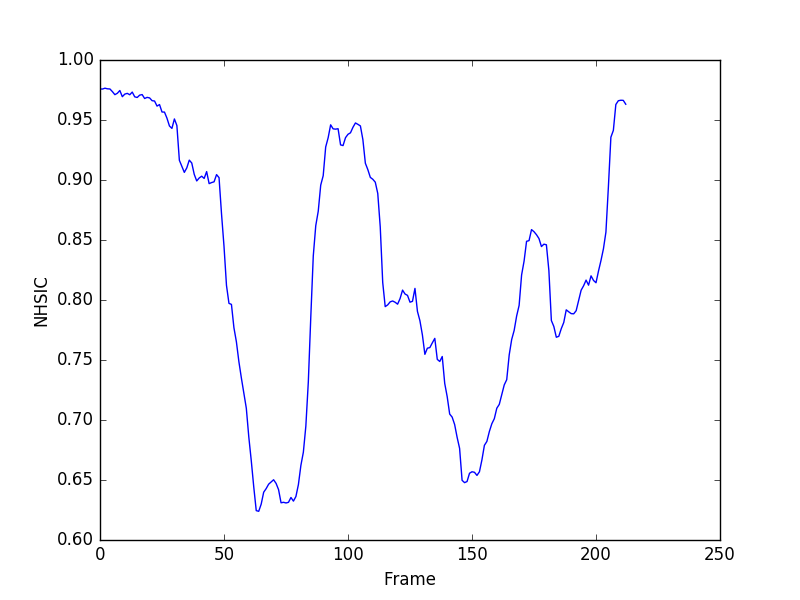
\includegraphics[width=\textwidth]{/home/cshome/j/jcampbell/Desktop/Thesis/Thesis/images/ts_08.png}
\caption{\label{ts_08}}
\end{figure}


\begin{figure}[h]
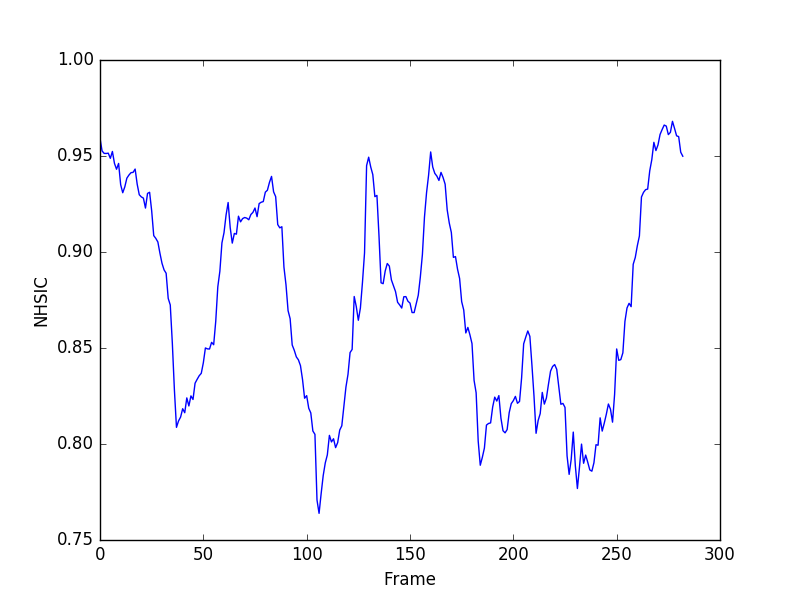
\includegraphics[width=\textwidth]{/home/cshome/j/jcampbell/Desktop/Thesis/Thesis/images/ts_10.png}
\caption{\label{ts_10}}
\end{figure}

\begin{figure}[h]
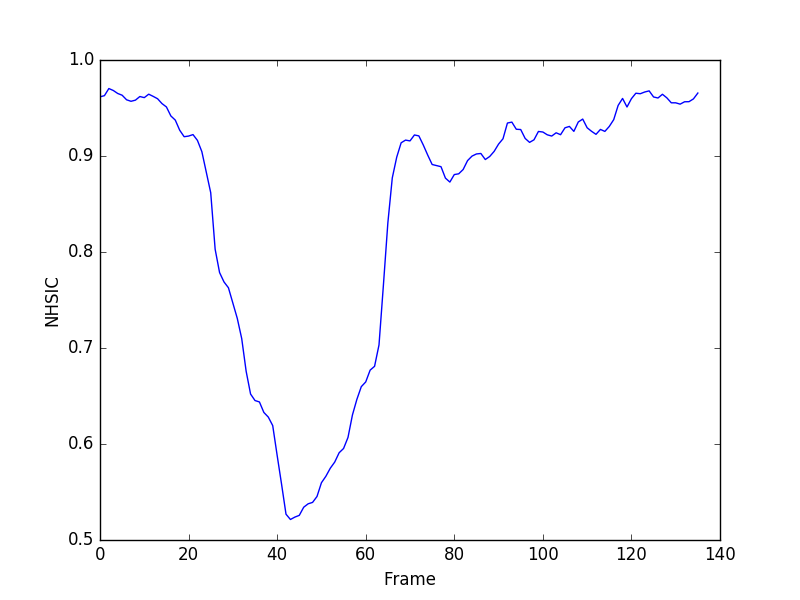
\includegraphics[width=\textwidth]{/home/cshome/j/jcampbell/Desktop/Thesis/Thesis/images/ts_11.png}
\caption{\label{ts_11}}
\end{figure}




























\section{Temporal Synchronisation}

There are often times when two vides of an activity will not be temporally aligned, for example in film making. In the film industry the term \textit{shot} is used to denote a short sequence of continuous activity which is not broken by a cut, typically on the order of 1000 frames. It is common for multiple cameras to record each shot, as well as infrared cameras if motion capture technology is being employed. Motion capture systems typically contain their own dedicated hardware temporal synchronisation frameworks, while an additional hardware synchronisation system is employed for the remaining cameras. Hardware synchronisation methods are occasionally used for filming outdoors, however they are often costly and require time to setup for each shoot. Hardware synchronisation methods are therefore inaccessible for amateur cinematographers, and for unplanned, ad hoc recording scenarios. In these situations it is therefore highly likely that the activity recorded from each camera will not be synchronised in time. Furthermore, even if hardware synchronisation has been used, once a shot has been captured it will often be sent to an editorial team, who may perform alterations to the shot which renders the timestamps incorrect. The original and the modified shots will therefore require manual synchronisation to align them again. Manual synchronisation is typically performed by searching for high frequency events such as footfalls, eyeblinks, or when any two items connect. This obviously introduces problems when there is very little scene activity, or when there are no high frequency components. This could occur in tracking shots that produce a sweeping motion, or for shots in which any activity is very smooth, for example a car driving along a street. \\

It is vitally important that multiple views of a shot are aligned in time. In live action films it is critical to know when to be able to switch between views, while in films that contain visual effects elements the multiple views are used as input to motion reconstruction pipelines, stereo reconstruction pipelines, and as raw input for artists manually creating creatures and scenes. \\

\subsection{Matching mocap with Iimage data}

One of the strengths of the HSIC is it can theoretically find all the functional dependencies between two random variables. Critically, this means that we can use the HSIC to match data from disparate sensing modalities, i.e. between mocap data and image data. In some film production settings it may be necessary to find the temporal offset between the motion capture data of a scene, and some video of that scene. We therefore tested our algorithm under these settings, and show that it is possible to synchronise 

\section{Activity Clustering}

\subsection{}


% \chapter{Introduction}
\label{chap:intro}

This is the first chapter.  Here is an example citation:
\citet{rountree98}.


% \chapter{Literature Survey}
\label{chap:lit}


% \chapter{A New Approach}
\label{chap:new}


% \chapter{Implementation}
\label{chap:implementation}


% \chapter{Results}
\label{chap:results}


% \chapter{Conclusion}
\label{chap:conclusion}


%%
%% Make certain the ``references'' section begins on a recto page when
%% document is double-sided.
%% The ``bibliography'' line assumes that there is a file called
%% ``thesis.bib'' and that somewhere in the chapter material you have
%% cited something from it.
%%
\cleardoublepage
\bibliographystyle{otago}
\bibliography{thesis}

%%
%% Now we have to get the source code in as a set of Appendices.
%% Source code will be Appendix A, with each file numbered X.y
%%
\appendix

%%
%% -> \chapter will cause the next bit to be labelled Appendix A
%% -> \section will give us A.1, \subsection A.1.1 etc.
%%
%% I suggest a section for each program and a subsection for each file
%% in the program.  Alternatively, a chapter for each program, a
%% section for each library and a subsection for each file.
%%
\chapter{Source Code for thesis.dvi}

\linespread{1}
\footnotesize

\section{thesis.tex}
\listinginput[10]{1}{thesis.tex}

\subsection{abstract.tex}
\listinginput[10]{1}{abstract.tex}

\subsection{acknowledgements.tex}
\listinginput[10]{1}{acknowledgements.tex}

\subsection{intro.tex}
\listinginput[10]{1}{intro.tex}

\subsection{literature.tex}
\listinginput[10]{1}{literature.tex}

\subsection{new\_ideas.tex}
\listinginput[10]{1}{new_ideas.tex}

\subsection{implementation.tex}
\listinginput[10]{1}{implementation.tex}

\subsection{results.tex}
\listinginput[10]{1}{results.tex}

\subsection{conclusion.tex}
\listinginput[10]{1}{conclusion.tex}

\subsection{appendices.tex}
\listinginput[10]{1}{appendices.tex}

%%
%% \listinginput[x]{y}{filename} gives a listing of <filename>,
%% starting at line y with a line-number at every xth line.
%%


\end{document}
%% All Done!
